% concatenated from cpCM_1_.tex
\documentclass[12pt]{amsart}
\usepackage[utf8]{inputenc}
\usepackage{bm}
\usepackage[dvipsnames,svgnames,x11names]{xcolor}
\usepackage[hyphens]{url}
\usepackage[colorlinks=true,
            linkcolor=Maroon,
            citecolor=blue,
            urlcolor=blue,
            hypertexnames=false,
            linktocpage]{hyperref}
\pdfstringdefDisableCommands{%
  \def\theta{theta}%
  \def\pi{pi}%
  \def\in{in }%
}
\usepackage{bookmark}
\usepackage{amsmath,thmtools,mathtools}
\usepackage{amssymb}
\mathtoolsset{showonlyrefs=true}
\usepackage{graphicx}
\usepackage{tikz}
\usepackage{tikz-3dplot}
\usetikzlibrary{arrows.meta,calc,intersections}
\usepackage{fancyhdr}
\usepackage{esint}
\usepackage{enumerate}
\usepackage{caption}
\setlength{\overfullrule}{5pt}
\allowdisplaybreaks



% ------------------ Custom commands ------------------
\newcommand{\bigslant}[2]{{\raisebox{.2em}{$#1$}\left/\raisebox{-.2em}{$#2$}\right.}}
\newcommand{\mres}{\mathbin{\vrule height 1.6ex depth 0pt width 0.13ex\vrule height 0.13ex depth 0pt width 1.3ex}}
\newcommand{\measurerestr}{\raisebox{.127ex}{\reflectbox{\rotatebox[origin=br]{-90}{$\lnot$}}}}

% Theorems
\declaretheorem[name=Theorem,numberwithin=section]{thm}
\declaretheorem[name=Remark,style=remark,sibling=thm]{rem}
\declaretheorem[name=Lemma,sibling=thm]{lemma}
\declaretheorem[name=Proposition,sibling=thm]{prop}
\declaretheorem[name=Definition,style=definition,sibling=thm]{defn}
\declaretheorem[name=Corollary,sibling=thm]{cor}
\declaretheorem[name=Question,sibling=thm]{qu}
\declaretheorem[name=Assumption,style=definition,sibling=thm]{assum}
\declaretheorem[name=Example,style=remark,sibling=thm]{example}
\declaretheorem[name=Notation,style=definition,sibling=thm]{nota}
\declaretheorem[name=Theorem,numbered=no]{theorem}
\declaretheorem[name=Corollary,numbered=no]{corollary}
\declaretheorem[name=Question,numbered=no]{question}
\declaretheorem[style=remark,name=Remark,numbered=no]{remark}
\declaretheorem[style=definition,name=Definition,numbered=no]{definition}
\declaretheorem[style=definition,name=Notation,numbered=no]{notation}
\declaretheorem[name=Lemma,numbered=no]{lem}
\numberwithin{equation}{section}

% ------------------ Math symbols ------------------
\newcommand{\OP}{\Lambda_p^{\phi}}
\newcommand{\Op}{\Lambda_p}
\newcommand{\ti}{\tilde}
\newcommand{\wt}{\widetilde}
\newcommand{\wh}{\widehat}
\newcommand{\bs}{\backslash}
\newcommand{\cn}{\colon}
\newcommand{\sub}{\subset}
\newcommand{\ov}{\overline}
\newcommand{\mr}{\mathring}
\newcommand{\bbN}{\mathbb{N}}
\newcommand{\bbZ}{\mathbb{Z}}
\newcommand{\bbQ}{\mathbb{Q}}
\newcommand{\bbR}{\mathbb{R}}
\newcommand{\bbC}{\mathbb{C}}
\newcommand{\bbS}{\mathbb{S}}
\newcommand{\bbH}{\mathbb{H}}
\newcommand{\bbK}{\mathbb{K}}
\newcommand{\bbD}{\mathbb{D}}
\newcommand{\bbB}{\mathbb{B}}
\newcommand{\bbE}{\mathbb{E}}
\newcommand{\bbM}{\mathbb{M}}
\newcommand{\M}{\mathcal{M}}
\newcommand{\W}{\mathcal{W}}
\newcommand{\Rn}{\mathbb{R}^{n+1}}
\newcommand{\Sn}{\mathbb{S}^n}
\newcommand{\op}[1]{\operatorname{#1}}
\newcommand{\8}{\infty}

% Greek
\newcommand{\al}{\alpha}
\newcommand{\be}{\beta}
\newcommand{\ga}{\gamma}
\newcommand{\de}{\delta}
\newcommand{\ep}{\epsilon}
\newcommand{\ka}{\kappa}
\newcommand{\la}{\lambda}
\newcommand{\om}{\omega}
\newcommand{\si}{\sigma}
\newcommand{\Si}{\Sigma}
\newcommand{\ph}{\phi}
\newcommand{\vp}{\varphi}
\newcommand{\ze}{\zeta}
\newcommand{\vt}{\vartheta}
\newcommand{\Om}{\Omega}
\newcommand{\De}{\Delta}
\newcommand{\Ga}{\Gamma}
\newcommand{\Th}{\Theta}
\newcommand{\La}{\Lambda}
\newcommand{\Ph}{\Phi}
\newcommand{\Ps}{\Psi}

% Mathcal
\newcommand{\cA}{\mathcal{A}}
\newcommand{\cB}{\mathcal{B}}
\newcommand{\cC}{\mathcal{C}}
\newcommand{\cD}{\mathcal{D}}
\newcommand{\cE}{\mathcal{E}}
\newcommand{\cF}{\mathcal{F}}
\newcommand{\cG}{\mathcal{G}}
\newcommand{\cH}{\mathcal{H}}
\newcommand{\cI}{\mathcal{I}}
\newcommand{\cJ}{\mathcal{J}}
\newcommand{\cK}{\mathcal{K}}
\newcommand{\cL}{\mathcal{L}}
\newcommand{\cM}{\mathcal{M}}
\newcommand{\cN}{\mathcal{N}}
\newcommand{\cO}{\mathcal{O}}
\newcommand{\cP}{\mathcal{P}}
\newcommand{\cQ}{\mathcal{Q}}
\newcommand{\cR}{\mathcal{R}}
\newcommand{\cS}{\mathcal{S}}
\newcommand{\cT}{\mathcal{T}}
\newcommand{\cU}{\mathcal{U}}
\newcommand{\cV}{\mathcal{V}}
\newcommand{\cW}{\mathcal{W}}
\newcommand{\cX}{\mathcal{X}}
\newcommand{\cY}{\mathcal{Y}}
\newcommand{\cZ}{\mathcal{Z}}

% Operators
\DeclareMathOperator{\dive}{div}
\DeclareMathOperator{\id}{id}
\DeclareMathOperator{\pr}{pr}
\DeclareMathOperator{\Diff}{Diff}
\DeclareMathOperator{\supp}{supp}
\DeclareMathOperator{\graph}{graph}
\DeclareMathOperator{\osc}{osc}
\DeclareMathOperator{\const}{const}
\DeclareMathOperator{\dist}{dist}
\DeclareMathOperator{\loc}{loc}
\DeclareMathOperator{\tr}{tr}
\DeclareMathOperator{\Rm}{Rm}
\DeclareMathOperator{\Rc}{Rc}
\DeclareMathOperator{\Sc}{R}
\DeclareMathOperator{\grad}{grad}
\DeclareMathOperator{\ad}{ad}
\DeclareMathOperator{\argmax}{argmax}
\DeclareMathOperator{\vol}{vol}
\DeclareMathOperator{\Area}{Area}
\DeclareMathOperator{\sgn}{sgn}
\DeclareMathOperator{\Rad}{Rad}
\DeclareMathOperator{\nul}{null}
\DeclareMathOperator{\ind}{ind}
\DeclareMathOperator{\diam}{diam}
\DeclareMathOperator{\sym}{sym}

% Shortcuts
\newcommand{\INT}{\int_{\Omega}}
\newcommand{\DINT}{\int_{\partial\Omega}}
\newcommand{\Int}{\int_{-\infty}^{\infty}}
\newcommand{\del}{\partial}
\newcommand{\n}{\nabla}
\newcommand{\II}[2]{\mathrm{II}(#1,#2)}
\newcommand{\fa}{\forall}
\newcommand{\rt}{\sqrt}
\newcommand{\ip}[2]{\langle #1,#2 \rangle}
\newcommand{\fr}[2]{\frac{#1}{#2}}
\newcommand{\tfr}[2]{\tfrac{#1}{#2}}
\newcommand{\x}{\times}
\newcommand{\br}[1]{(#1)}
\newcommand{\abs}[1]{\lvert #1\rvert}

% Environments
\newcommand{\pf}[1]{\begin{proof}#1\end{proof}}
\newcommand{\eq}[1]{\begin{equation}\begin{alignedat}{2}#1\end{alignedat}\end{equation}}

% Capillary setup
\newcommand{\Rplus}{\bbR^{n+1}_+}
\newcommand{\Cth}{\cC_\theta}
\newcommand{\bn}{\nabla}
\newcommand{\bHess}{\nabla^2}
\newcommand{\Sd}{\mathbb{S}^{d-1}}
\newcommand{\Hd}{\mathcal{H}}
\newcommand{\R}{\mathbb{R}}


% Page geometry
\oddsidemargin 0.6in
\evensidemargin 0.6in
\textwidth 5.5in

\begin{document}

\title{Capillary $L_p$-Christoffel-Minkowski problem}
	\author[Y. Hu, M. N. Ivaki]{Yingxiang Hu, Mohammad N. Ivaki}

\begin{abstract}
We solve the capillary $L_p$-Christoffel--Minkowski problem in the half-space for $1<p<k+1$ in the class of even hypersurfaces. A crucial ingredient is a non-collapsing estimate that yields lower bounds for both the height and the capillary support function. Our result extends the capillary Christoffel--Minkowski existence result of \cite{HIS25}.
\end{abstract}

\maketitle

\section{Introduction}
The problem of prescribing area measures of convex hypersurfaces originates in the classical works of Christoffel \cite{Chr65}, Minkowski \cite{Min97,Min03}, Aleksandrov \cite{Ale56}, Nirenberg \cite{Nir57} and Pogorelov \cite{Pog52,Pog71}, which established the modern interplay between convex geometry and fully nonlinear elliptic equations. In the smooth setting, the Christoffel--Minkowski problem seeks a smooth, strictly convex hypersurface whose $k$-th elementary symmetric function of the principal radii of curvature agrees with a given function on the sphere. This direction was further developed in the works of Firey and Berg \cite{Fir67,Fir70,Ber69}.

Over the past decades, the Christoffel--Minkowski problem has seen substantial progress. For the top-order case $k=n$, corresponding to the classical Minkowski problem, the situation is by now well understood: the seminal works of Cheng--Yau \cite{CY76} and Caffarelli \cite{Caf90a,Caf90b} provide an existence and regularity theory for the underlying fully nonlinear equation. For intermediate orders $1< k<n$, the picture is less complete, although \cite{GM03,STW04} provide a far-reaching existence result for the Christoffel--Minkowski problem in the smooth setting. See also \cite{BHOM25,MU25} for the recent break-through in the rotationally symmetric case. 

The $L_p$-extension of the Christoffel--Minkowski problem, introduced by Lutwak \cite{Lut93} in the framework of the Brunn--Minkowski--Firey theory, replaces the classical area measures by their $L_p$ analogues and leads to the curvature equation
\eq{
  \si_k(\tau^\sharp[h]) = h^{p-1}\phi \quad \text{on }\bbS^n,
}
for the support function $h$ of a smooth, strictly convex body/hypersurface, where $\tau^\sharp[h]=g^{-1}\cdot(\nabla^2 h+h g)$ and $g$ denotes the standard metric on $\bbS^n$. The $L_p$-Minkowski problem has since been the subject of intensive study and has developed into a mature theory over a broad range of $p$; see \cite{LO95,CW06,BLYZ13,HLYZ16,BBCY19,HXZ21,GLW22,LXYZ24} and also \cite{CW00,BIS19,LWW20,CL21,BIS21b,BG23}. In contrast, for $k<n$ the situation is more fragmentary as  the intermediate $L_p$-area measures remain, in general, much less understood. In the smooth case, however, and in particular for $p>1$ with even data on $\bbS^n$, one now has a well-developed set of results: existence, uniqueness and regularity of solutions, together with constant rank theorems ensuring strict convexity; see, for instance, \cite{GM03,HMS04,GLM06,GMZ06,GX18,Iva19,BIS23,BIS23b,HI24,Zha24,CH25} and \cite{BIS21,HLX24,LW24}.

A natural question is how this picture changes in the presence of a boundary. In the capillary setting, one considers hypersurfaces in the half-space that meet a fixed supporting hyperplane at a prescribed contact angle $\theta\in(0,\pi/2)$. For the top-order case $k=n$, capillary versions of the $L_p$-Minkowski problem have been developed in a series of recent works. For $p\ge 1$, Mei, Wang and Weng solved the capillary $L_p$-Minkowski problem via the continuity method in \cite{MWW25a,MWW25c}. For $-(n+1)<p<1$, even solutions were constructed in \cite{HI25} by means of an iterative scheme based on the curvature image operator, and a unified curvature flow approach was later introduced in \cite{HHI25}, treating the even capillary $L_p$-Minkowski problem for all $p>-(n+1)$.

For $ k<n$, the capillary analogue of the Christoffel--Minkowski problem prescribes $\si_k(\tau^\sharp[s])$ on the capillary spherical cap $\Cth$ and couples the interior equation with a Robin boundary condition encoding the contact angle. This capillary analogue was solved in \cite{HIS25}, where the existence of smooth, strictly convex, $\theta$-capillary hypersurfaces was established under conditions on the prescribed function that are tailored to the applicability of a constant rank theorem. The existence of a solution to the capillary Christoffel-Minkowski problem was also established in \cite{MWW25c}, subject to an additional assumption concerning the existence of a suitable homotopy path.

The aim of this paper is to extend the work \cite{HIS25} to the $L_p$-framework in the range $1<p<k+1$. In analogy with the closed case \cite{GM03,GX18}, we study the prescribed curvature equation
\eq{
  \si_k(\tau^\sharp[s]) = s^{p-1}\phi
  \quad\text{in }\Cth
}
for an even, positive, smooth function $\phi$ on $\Cth$, together with the capillary boundary condition
\eq{
  \n_\mu s = \cot\theta\,s
  \quad\text{on }\partial\Cth.
}

\begin{thm}\label{thm:main}
Let $1 < p < k+1$, $\theta \in (0, \pi/2)$, and $\phi \in C^\infty(\mathcal{C}_\theta)$ be a positive function satisfying
\eq{
\phi(-\zeta_1,\ldots,-\zeta_n,\zeta_{n+1})=\phi(\zeta_1,\ldots,\zeta_n,\zeta_{n+1})\quad \forall \zeta\in \Cth,
}
\eq{\label{spherically-convex}
\nabla^2\phi^{-\frac{1}{p+k-1}} + g\phi^{-\frac{1}{p+k-1}} \ge 0 \quad \text{in }\Cth
}
and the boundary condition
\eq{ \label{bdry-condition}
\nabla_\mu\phi^{-\frac{1}{p+k-1}} \le \cot\theta \,\phi^{-\frac{1}{p+k-1}} \quad \text{on } \partial\mathcal{C}_\theta.
}
Then there exists a unique even, strictly convex, capillary hypersurface $\Sigma \subset \overline{\mathbb{R}^{n+1}_+}$ with contact angle $\theta$ whose capillary support function $s$ solves
\eq{\label{capillary-Lp-eq}
\left\{
\begin{aligned}
  \sigma_k(\tau^\sharp[s])
    &= s^{p-1} \phi
    &&\text{in }\Cth,\\
  \nabla_\mu s &= \cot\theta\,s
    &&\text{on }\partial\Cth.
\end{aligned}
\right.
}
\end{thm}

The paper is organized as follows. In Section \ref{sec:preliminaries} we recall the basic capillary geometry in the half-space and fix notation. Section \ref{sec:non-collapsing} is devoted to non-collapsing estimates; i.e. a lower bound for the height of the hypersurface, both in the rotationally symmetric and in the general even case. In Section \ref{sec:regularity} we derive curvature and regularity estimates for solutions of \eqref{capillary-Lp-eq}. In Section \ref{sec:strict-convexity} we prove a capillary constant rank theorem for our equation. Finally, in Section \ref{sec:existence-uniqueness} we complete the proof of \autoref{thm:main} by establishing existence and uniqueness.

\section{Preliminaries}\label{sec:preliminaries}
Let $\{e_i\}_{i=1}^{n+1}$ be the standard orthonormal basis of $\bbR^{n+1}$. Let 
\eq{
\mathbb{R}^{n+1}_+ = \{x \in \mathbb{R}^{n+1}: x_{n+1} > 0\}
}
be the upper half-space with boundary $\partial\mathbb{R}^{n+1}_+ = \{x_{n+1} = 0\}$. The unit ball of $\bbR^{n+1}$ is denoted by $\bbB$, and we write $\bbS^n$ for the unit ball.

\begin{enumerate}[(1)]
\item \textbf{Support functions of convex bodies.}
For a bounded convex set $K\subset\bbR^{n+1}$, the support function
$h_K:\Sn\to\bbR$ is defined as
\eq{
  h_K(u):=\sup\{\langle x,u\rangle:x\in K\},\quad u\in\Sn.
}
When no confusion can arise, we simply write $h:=h_K$.

\item \textbf{Area measures in $\bbR^{n+1}$.}
Let $K\subset\bbR^{n+1}$ a bounded convex set and $k\in\{0,\dots,n\}$. The $k$-th area measure $S_k(K,\cdot)$ is the finite Borel measure on $\Sn$ appearing in the classical local Steiner formula. If $K$ is smooth and strictly convex with principal radii of curvature $\la_1,\dots,\la_n$ at a point with outer unit normal $u\in\Sn$, then
\eq{
  dS_k(K,u)
  = \frac{1}{\binom{n}{k}}
    \sigma_k(\la_1,\dots,\la_n)\,d\si(u),
}
where $d\si$ denotes the spherical Lebesgue measure on $\Sn$.
If $L\subset\bbR^{n+1}$ is an $m$-dimensional linear subspace and
$K\subset L$, we write $S_k^L(K,\cdot)$ for the $k$-th area measure of
$K$ viewed as a convex set in $L$.

\item \textbf{Hausdorff measure and subspheres.}
For any integer $d\ge 1$, we write $\Hd^d$ for the $d$-dimensional Hausdorff measure, and
\eq{
  \bbS^d := \{x\in\R^{d+1} : |x|=1\}
}
for the unit sphere in $\R^{d+1}$. For a linear subspace
$L\subset\R^{n+1}$ of dimension $m$, we identify $\Sn\cap L$ with the unit sphere in $L$.
We also write
\eq{
  \mathbb{S}^n_\theta := \{x\in\Sn : \langle x,e_{n+1}\rangle \ge \cos\theta\}, \quad \cC_{\theta}:=\bbS^n_{\theta}-\cos\theta\, e_{n+1}.
}

Integrals of the form
\eq{
  \int_{\Sn} f,\quad
  \int_{\mathbb{S}^n_\theta} f,\quad
  \int_{\Cth} f,\quad
  \int_{\Sn\cap L} f,\quad
  \int_{\bbS^d} f,
}
are always understood with respect to the restriction of the appropriate Hausdorff measure
(thus, $\Hd^n$ on $\Sn$, $\mathbb{S}^n_\theta$ and $\Cth$, $\Hd^{m-1}$ on $\Sn\cap L$, and $\Hd^{d}$ on $\bbS^d$).
We also write
\eq{
  \omega_d := \Hd^{d}(\mathbb{S}^d),
}
so that $\omega_d$ is the surface area of $\mathbb{S}^d$.
\end{enumerate}


\begin{defn}
A smooth, compact, connected, orientable hypersurface $\Sigma \subset \overline{\mathbb{R}^{n+1}_+}$ with $\mathrm{int}(\Sigma) \subset \mathbb{R}^{n+1}_+$ and $\partial\Sigma \subset \partial\mathbb{R}^{n+1}_+$ is called a capillary hypersurface with contact angle $\theta \in (0,\pi)$ if
\eq{
\langle \nu, e_{n+1} \rangle = \cos\theta \quad \text{on } \partial\Sigma,
}
where $\nu$ is the outer unit normal of $\Sigma$.
\end{defn}

The model capillary surface is
\eq{
\mathcal{C}_\theta
 = \{\zeta \in \overline{\mathbb{R}^{n+1}_+} : |\zeta + \cos\theta\, e_{n+1}| = 1\}.
}
Via the translation
\eq{
T(\zeta) := \zeta + \cos\theta\,e_{n+1},
}
we may identify \(\mathcal{C}_\theta\) with \(\mathbb{S}^n_\theta\).

We also define
\eq{
\mathcal{C}_{\theta, r} := \left\{ \zeta \in \overline{\mathbb{R}_+^{n+1}} \mid |\zeta + r \cos \theta\, e_{n+1}| = r \right\}.
}
Note that the radius of $\partial \mathcal{C}_{\theta, r}$ is $r\sin\theta$.

We call $\Si$ strictly convex if the enclosed region $\widehat\Si$ is a convex body (i.e. compact, convex, with non-empty interior) and the second fundamental form of $\Si$ is positive definite. For a strictly convex capillary hypersurface $\Sigma$, the capillary Gauss map is defined as
\eq{
\tilde{\nu} = \nu - \cos\theta\, e_{n+1}: \Sigma \to\Cth.
}
This is a diffeomorphism onto the capillary spherical cap, see \cite[Lem. 2.2]{MWWX25}.

\begin{defn}
Let $\Si$ be a strictly convex, capillary hypersurface. The capillary support function $s:\Cth \to \mathbb{R}$ of $\Sigma$ is defined by
\eq{
s(\zeta) = \langle \tilde{\nu}^{-1}(\zeta), \zeta + \cos\theta\, e_{n+1} \rangle.
}
\end{defn}

For the model cap $\mathcal{C}_\theta$, the capillary support function is
\eq{
\ell(\zeta) = \sin^2\theta - \cos\theta\langle \zeta, e_{n+1} \rangle.
}

On $\Cth$ we also write $g$ for the round metric, $\nabla$ for its
Levi-Civita connection and $\nabla^2$ for the covariant Hessian.
For a function $f\in C^2(\Cth)$ we set
\eq{
  \tau[f]:=\nabla^2 f+f\,g,\quad
  \tau^\sharp[f]:=g^{-1}\cdot\tau[f],
}
so that $\tau^\sharp[f]$ is a symmetric endomorphism of $T\Cth$. Its
eigenvalues are denoted by $\la_1,\dots,\la_n$, and
$\sigma_k(\tau^\sharp[f])$ means $\sigma_k(\la_1,\dots,\la_n)$.
We also write $\nabla_\mu f$ for the covariant derivative in the
direction of the outward unit conormal $\mu$ along $\partial\Cth$.


For a symmetric matrix $A=(a_{ij})$ with eigenvalues
$\la_1,\dots,\la_n$ we write
\eq{
  \sigma_k^{ij}(A):=\frac{\partial\sigma_k}{\partial a_{ij}}(A),
}
and for $F=\sigma_k^{1/k}$ we set
\eq{
  F^{ij}(A):=\frac{\partial F}{\partial a_{ij}}(A)
           =\frac1k\,\sigma_k(A)^{\frac{1}{k}-1}\sigma_k^{ij}(A).
}
When $A=\tau^\sharp[s]$ for some function $s$ on $\Cth$, we abbreviate
$\sigma_k^{ij}(\tau^\sharp[s])$ and $F^{ij}(\tau^\sharp[s])$ by
$\sigma_k^{ij}$ and $F^{ij}$, respectively.


Writing points of $\Rn$ as $x=(x_1,\dots,x_n,x_{n+1})$, let $\cR$ denote the reflection
\eq{
  \cR(x_1,\dots,x_n,x_{n+1})
  := (-x_1,\dots,-x_n,x_{n+1}).
}
A function $\varphi:\Cth\to\bbR$ is called even if $\varphi\circ\cR=\varphi$, and we say that a capillary hypersurface $\Si$ (or its capillary support function $s$) is even if
\eq{
  x\in\Si
  \implies
   \cR(x)\in\Si.
}

\begin{defn}\label{def:mixed-volume}
Let $k\in\{0,\dots,n\}$. Let $s_0,\dots,s_{n}\in C^\infty(\Cth)$ be capillary
support functions. Denote by $Q_k$ the linear polarization of
$\sigma_k$ on symmetric endomorphisms of $T\Cth$, i.e. the unique symmetric
multilinear map such that
\eq{
  Q_k(A,\dots,A)=\frac{\sigma_k(A)}{\binom{n}{k}}
  \quad\text{for every symmetric endomorphism }A.
}
The capillary mixed volume of $s_0,\dots,s_{k}$ is defined by
\eq{\label{def:Vk}
  V(s_0,\dots,s_{k},\underbrace{\ell,\ldots,\ell}_{(n-k)-\text{times}})
  := \frac{1}{n+1}
     \int_{\Cth}
       s_0
       Q_k\bigl(
         \tau^\sharp[s_1],\dots,\tau^\sharp[s_{k}],
         \underbrace{\tau^\sharp[\ell],\dots,\tau^\sharp[\ell]}_{(n-k)-\text{times}}
       \bigr).
}
In particular, one has
\eq{\label{eq:Vk-special}
  V(s_0,\underbrace{s,\dots,s}_{k- \text{times}},\ell,\dots,\ell)
  = \frac{1}{n+1}\int_{\Cth} s_0\frac{\sigma_k\bigl(\tau^\sharp[s]\bigr)}{\binom{n}{k}}.
}
\end{defn}

\begin{thm}\label{lem:tilde-nu-parallel body}
Let $\Sigma\subset\ov{\bbR^{n+1}_+}$ be a strictly convex, $\theta$-capillary hypersurface.
For $t>0$ define
\eq{ \phi_t:\Sigma\to\ov{\bbR^{n+1}_+},\quad \phi_t(x):=x+t \tilde\nu(x).
}
Then $\Sigma_t:=\phi_t(\Sigma)$ is a strictly convex, $\theta$-capillary hypersurface. Moreover, the (standard) outer parallel convex body
\eq{
  K_t:=\bigl(\widehat{\Sigma}-t\cos\theta\,e_{n+1}\bigr)+t\,\bbB,
}
and the capillary outer parallel convex body are related via $\wh{\Si_t}=K_t\cap \ov{\bbR^{n+1}_+}$.
In addition, we have $\Si_t=\Si+t\Cth$.
\end{thm}

\begin{proof}
Let $P=\{x_{n+1}=0\}$. Define $f(x)=\langle x,e_{n+1}\rangle=x_{n+1}$ and
\eq{
  g(x)=\langle \tilde\nu(x),e_{n+1}\rangle
       =\langle \nu(x),e_{n+1}\rangle-\cos\theta.
}
Then
\eq{\label{eq:height-after-shift}
  \langle \phi_t(x),e_{n+1}\rangle = f(x)+t\,g(x).
}   

\emph{Step 1.}
On $\partial\Sigma$ we have $f=0$ (since $\partial\Sigma\subset P$) and $g=0$ (by capillarity),
hence $(f+tg)(x)=0$ for $x\in\partial\Sigma$, i.e. $\phi_t(\partial\Sigma)\subset P$. Moreover, since $\nu(\op{int}(\Si))\subset \op{int}(\bbS^n_{\theta})$, $f+t g>0$ on $\op{int}(\Sigma)$ for any $t>0$. 

\emph{Step 2.}
Let $x\in\Sigma$ and choose an orthonormal basis $\{e_1,\dots,e_n\}$ of $T_x\Sigma$
consisting of principal directions, so that
\eq{
  {}^{\Si}\nabla_{e_i}\nu=\kappa_i e_i,\quad i=1,\dots,n,
}
with principal curvatures $\kappa_i$.
We have ${}^{\Si}\nabla_{e_i}\tilde\nu={}^{\Si}\nabla_{e_i}\nu$, and therefore
\eq{
  d\phi_t(e_i)=e_i+t\,{}^{\Si}\nabla_{e_i}\tilde\nu
  =e_i+t\,{}^{\Si}\nabla_{e_i}\nu
  =(1+t\kappa_i)e_i.
}
Thus $d\phi_t(T_x\Sigma)$ is spanned by $\{e_1,\dots,e_n\}$, $\phi_t$ is a smooth immersion, and the oriented unit normal of $\Sigma_t=\phi_t(\Sigma)$
at $y=\phi_t(x)$ equals $\nu(x)$, i.e.
\eq{
  \nu_t(y)=\nu(x)\quad\text{for }y=\phi_t(x).
}
Next we show that $\phi_t$ is an injective immersion and thus an embedding. Assume $\phi_t(x)=\phi_t(x')$ for some
$x,x'\in\Sigma$. Then
\eq{
  x+t(\nu(x)-\cos\theta\,e_{n+1})=x'+t(\nu(x')-\cos\theta\,e_{n+1}),
}
hence
\eq{\label{eq:inj-start}
  x-x'=t\bigl(\nu(x')-\nu(x)\bigr).
}
Taking the inner product with $\nu(x)$ gives
\eq{\label{eq:inj-ip}
  \ip{x-x'}{\nu(x)}=t\bigl(\ip{\nu(x')}{\nu(x)}-1\bigr).
}
Since $\wh{\Si}$ is convex and $\nu(x)$ is the outer normal vector to $\Si$ at $x$,
\eq{
  \ip{x'-x}{\nu(x)}\le 0.
}
On the other hand, $\ip{\nu(x')}{\nu(x)}\le 1$, hence by \eqref{eq:inj-ip}
\eq{
  \ip{x-x'}{\nu(x)}=0
  \quad\text{and}\quad
  \ip{\nu(x')}{\nu(x)}=1.
}
Thus $\nu(x')=\nu(x)$. Since $\Sigma$ is strictly convex, the Gauss map
$\nu:\Sigma\to\bbS_{\theta}^n$ is injective, hence $x'=x$.

\emph{Step 3.}
If $y=\phi_t(x)$ with $x\in\partial\Sigma$, then by step 1 and step 2 we have $y\in P$ and
$\nu_t(y)=\nu(x)$. Therefore,
\eq{
  \langle \nu_t(y),e_{n+1}\rangle
  = \langle \nu(x),e_{n+1}\rangle
  = \cos\theta,
}
so $\Sigma_t$ meets $P$ with the same contact angle $\theta$.


\emph{Step 4.}
Let $x\in\Sigma$ and set
\eq{
y:=\phi_t(x)=x+t(\nu(x)-\cos\theta\,e_{n+1}).
}
We claim that $y\in\partial K_t$ and that $\nu(x)$ is an outer normal of $K_t$ at $y$.

Note that $y\in K_t$. Since $\nu(x)$ is an outer unit normal of the convex body $\widehat{\Sigma}$ at $x$, we have
\eq{\label{eq:support-K}
  \ip{z-x}{\nu(x)}\le 0\quad\forall\,z\in \widehat{\Sigma}.
}
Let $w\in K_t$. Then for some $z\in \widehat{\Sigma}$ and $b\in\bbB$:
\eq{
  w=(z-t\cos\theta\,e_{n+1})+tb.
}
Moreover, we have
\eq{
  \ip{w-y}{\nu(x)} = \ip{z-x}{\nu(x)} + t\ip{b}{\nu(x)} - t.
}
Using \eqref{eq:support-K}, we obtain
\eq{
  \ip{w-y}{\nu(x)}\le 0\quad\forall\,w\in K_t.
}
Hence we must have $y\in\partial K_t$ and $\nu(x)$ is an outer normal of $K_t$ at $y$.

\emph{Step 5.} Let $L_t=K_t\cap\ov{\bbR^{n+1}_+}$.
We prove
\eq{
  \Sigma_t=\phi_t(\Sigma)\subset\partial L_t.
}

If  $x\in\op{int}(\Sigma)$, then by step 1, we have
\eq{
  y=\phi_t(x)\in\bbR^{n+1}_+.
}
Together with $y\in\partial K_t$ (by step 4) this implies $y\in\partial L_t\setminus P$.

If  $x\in\partial\Sigma$, then by step 1, $\phi_t(\partial\Sigma)\subset P$, so $y\in P$.
Let $x_j\in\op{int}(\Sigma)$ be any sequence with $x_j\to x$. Set $y_j:=\phi_t(x_j)$. By continuity, $y_j\to y$.
Since $y_j\in \partial L_t$ the limit point $y$ belongs to $\partial L_t\cap P$.

\emph{Step 6.}
We prove $ \ov{\partial L_t\setminus P}= \Sigma_t$. By steps 1, 2 and 5,
\eq{
  \op{int}(\Si_t)=\phi_t(\op{int}(\Si))\subset\partial L_t\setminus P\implies \Sigma_t \subset \ov{\partial L_t\setminus P}.
}
It remains to prove $\partial L_t\setminus P \subset \Sigma_t\setminus P$.


Let $y\in\partial L_t\setminus P$. Then $y\in\partial K_t$. Suppose $u\in\bbS^n$ is an outer unit normal to $K_t$ at $y$, i.e.
\eq{\label{eq:supporting-at-y}
  \ip{w-y}{u}\le 0\quad\forall\,w\in K_t.
}
We may write
\eq{\label{eq:y-decomposition}
  y=(x-t\cos\theta\,e_{n+1})+tb,
  \quad x\in \widehat{\Sigma},\quad b\in\bbB.
}
We claim that $b=u$, $x\in \partial \wh{\Si}$, and $u$ is an outer normal of $\widehat{\Sigma}$ at $x$. 

Indeed, take any $x_0\in \widehat{\Sigma}$ and any $c\in\bbB$, and set
\eq{
  w=(x_0-t\cos\theta\,e_{n+1})+tc\in K_t.
}
Plugging this $w$ and \eqref{eq:y-decomposition} into \eqref{eq:supporting-at-y} gives
\eq{
  0\ge \ip{w-y}{u}
  =\ip{x_0-x}{u}+t\ip{c-b}{u}.
}
With $x_0=x$ and $c=u$,
\eq{
  1\le \ip{b}{u}\implies b=u.
}
Now with $c=b=u$, the inequality becomes
\eq{
  0\ge \ip{x_0-x}{u}\quad\forall\,x_0\in \widehat{\Sigma},
}
so $x\in \partial \wh{\Si}$ and $u$ is an outer normal of $\widehat{\Sigma}$ at $x$.

Since $y_{n+1}>0$ and $t>0$, we have from \eqref{eq:y-decomposition} (with $b=u$)
\eq{
  y_{n+1}=x_{n+1}-t\cos\theta+tu_{n+1}>0.
}
This implies that $x_{n+1}>0$, $x\in \Si$ and $u=\nu(x)$ (otherwise, if $x_{n+1}=0$, then we would have $u_{n+1}\le \cos\theta$ and hence $y_{n+1}\le 0$).
Substituting $b=u=\nu(x)$ into \eqref{eq:y-decomposition} yields
\eq{
  y=x+t(\nu(x)-\cos\theta\,e_{n+1})=\phi_t(x)\in\Sigma_t\setminus P.
}

\emph{Step 7.} By the previous steps, $\Si_t$ is a strictly convex (i.e. the enclosed region $\wh{\Si_t}$ is a convex body and the second fundamental form of $\Si_t$ is positive definite), $\theta$-capillary hypersurface, and for each point $x\in \Sigma$, the outward unit normal at the point $\phi_t(x)\in\Sigma_t$ is $\nu(x)$. Let $\zeta=\nu(x)-\cos\theta\, e_{n+1}$. Then
\eq{
s_{\Sigma_t}(\zeta)&=\langle \phi_t(x),\nu(x)\rangle\\
&=\langle x+t(\nu(x)-\cos\theta e_{n+1}),\nu(x)\rangle\\
&=s_{\Sigma}(\zeta)+t\ell(\zeta),
}
Since $\Sigma_t$ has the same capillary support function as $\Sigma+t\Cth$, we conclude that
\eq{
  \Sigma_t=\Sigma+t\Cth.
}
\end{proof}
\begin{rem}
The notion of capillary outer parallel sets for the capillary convex bodies was first introduced in \cite{MWW25c}, while the relation $\Sigma_t=\Sigma+t\Cth$ was observed in \cite[Rem. 2.17]{MWWX25}. \autoref{lem:tilde-nu-parallel body} clarifies the connection between capillary and classical outer parallel hypersurfaces, see \autoref{fig:example}.
\end{rem}
\begin{figure}
\begin{center}
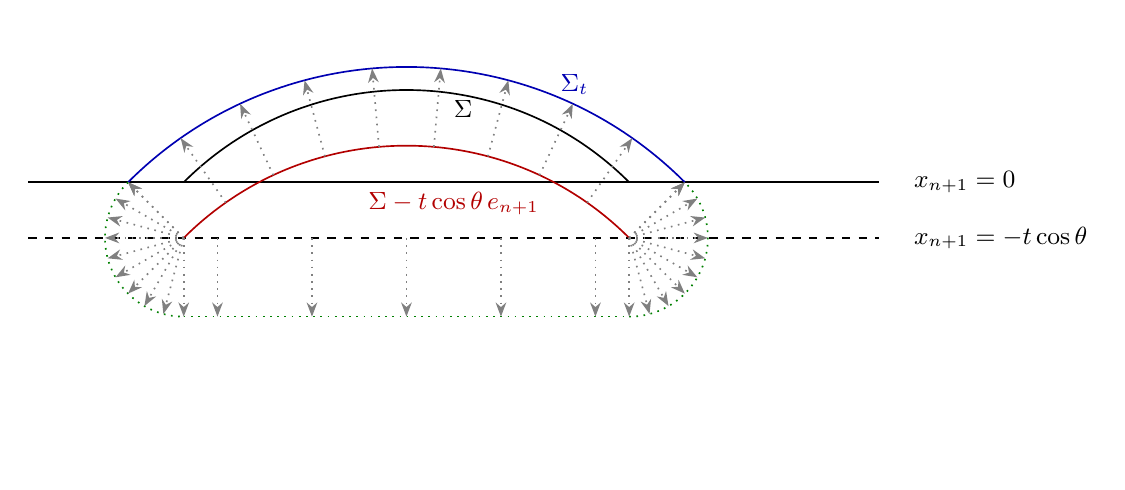
\begin{tikzpicture}[
  scale=4,
  semithick,
  font=\small,
  plane/.style={black},
  auxplane/.style={black, dashed},
  prored/.style={red!70!black},
  problue/.style={blue!70!black},
  progreen/.style={green!50!black, dotted}
]

  % parameters: theta = pi/4, t = 1/4
  \pgfmathsetmacro{\tval}{0.25}
  \pgfmathsetmacro{\cth}{sqrt(2)/2}          % cos(pi/4)
  \pgfmathsetmacro{\h}{\tval*\cth}           % h = t cos(theta)

  % unit radius
  \pgfmathsetmacro{\r}{1.0}
  \pgfmathsetmacro{\R}{\r+\tval}
  \pgfmathsetmacro{\a}{\r*sqrt(2)/2}

  % centers
  \coordinate (Cblk) at (0,-\a);
  \coordinate (Cred) at (0,{-\a-\h});

  % plane x_{n+1}=0
  \draw[plane] (-1.20,0) -- (1.50,0);
  \node[anchor=west] at (1.58,0) {$x_{n+1}=0$};

  % dashed line x_{n+1}=-t cos(theta)
  \draw[auxplane] (-1.20,-\h) -- (1.50,-\h);
  \node[anchor=west] at (1.58,-\h) {$x_{n+1}=-t\cos\theta$};

  % black curve: \Sigma
  \draw[black] (Cblk) ++(45:\r) arc (45:135:\r);

  % red curve: \Sigma - t cos(theta) e_{n+1} (arc only)
  \draw[prored] (Cred) ++(45:\r) arc (45:135:\r);

  % blue curve: \Sigma_t
  \draw[problue] (Cred) ++(45:\R) arc (45:135:\R);

  % green dotted pieces (exact offset at distance t)
  \coordinate (Rr) at (\a,-\h);
  \coordinate (Rl) at (-\a,-\h);

  \draw[progreen] (-\a,{-\h-\tval}) -- (\a,{-\h-\tval});
  \draw[progreen] (Rr) ++(-90:\tval) arc (-90:45:\tval);
  \draw[progreen] (Rl) ++(135:\tval) arc (135:270:\tval);

  % arrows: ALL have length t
  \begin{scope}[
    -{Stealth[scale=0.9]},
    draw=gray,
    dotted
  ]
    % along the red arc: radial normals (length t)
    \foreach \ang in {45,55,...,135} {
      \draw ($(Cred)+(\ang:\r)$) -- ($(Cred)+(\ang:\R)$);
    }

    % along the flat side y=-h: vertical normals (length t) -> reach green segment
    \foreach \xx in {-0.60,-0.30,0,0.30,0.60} {
      \draw (\xx,-\h) -- (\xx,{-\h-\tval});
    }

    % corner normal cones (length t)
    \foreach \ang in {-90,-75,...,45} {
      \draw (Rr) -- ($(Rr)+(\ang:\tval)$);
    }
    \foreach \ang in {135,150,...,270} {
      \draw (Rl) -- ($(Rl)+(\ang:\tval)$);
    }
  \end{scope}

  % labels (no arrows)
  \coordinate (LblBluePt) at ($(Cred)+(70:\R)$);
  \node[text=blue!70!black, anchor=west] at ($(LblBluePt)+(0.03,0.02)$) {$\Sigma_t$};

  \coordinate (TopBlk) at ($(Cblk)+(90:\r)$);
  \node[text=black, anchor=north] at ($(TopBlk)+(0.18,0.00)$) {$\Sigma$};

  \node[text=red!70!black, anchor=north] at (0.15,0.00)
    {$\Sigma-t\cos\theta\,e_{n+1}$};

\end{tikzpicture}
\caption{Capillary vs. classical outer parallel hypersurfaces}
\label{fig:example}
\end{center}
\end{figure} 

For $\rho>0$ and a Borel set $\omega\sub\Cth$,
the local outer parallel set of $\wh\Si$ in the directions of $\omega$ can be defined by
\eq{\label{eq:def-B-rho}
B_{\rho,\theta}(\wh\Si,\omega)
&:= \left\{y\in\ov{\Rplus}:
\begin{array}{l}
\exists x\in\Si,\, 0<t<\rho,\, \text{s.t.}\\
y=x+t\tilde{\nu}(x),\,\tilde{\nu}(x)\in\omega
\end{array}
\right\}.
}

\begin{lemma}\label{lem:local-Steiner}
Let $\Si\sub\ov{\Rplus}$ be a strictly convex $\theta$-capillary
hypersurface with principal curvatures
$\kappa=(\kappa_1,\dots,\kappa_n)$ and area element $d\mu$. Then, for every
Borel set $\omega\sub\Cth$ and every $\rho>0$,
\eq{\label{eq:local-Steiner-geom}
\vol\bigl(B_{\rho,\theta}(\wh\Si,\omega)\bigr)
=\sum_{j=0}^n \frac{\rho^{n+1-j}}{n+1-j}
\int_{\Si\cap\tilde{\nu}^{-1}(\omega)}
  \bigl(1-\cos\theta\ip{\nu}{e_{n+1}}\bigr)\si_{n-j}(\kappa)\,d\mu.
}
\end{lemma}
\begin{proof}
The local Steiner-type formula was previously stated in \cite{MWW25c}. For completeness, we give a proof here.
Let
\eq{
  \Phi:\Si\times(0,\infty)\to\ov{\Rplus},\quad
  \Phi(x,t):=x+t\tilde{\nu}(x).
}
By \autoref{lem:tilde-nu-parallel body}, $\Phi$ maps $\Si$ to  strictly convex, $\theta$-capillary hypersurfaces.

For a given Borel set $\omega\sub\Cth$, the definition
\eqref{eq:def-B-rho} gives
\eq{
  B_{\rho,\theta}(\wh\Si,\omega)
  = \Phi\Bigl(
        \bigl(\Si\cap\tilde{\nu}^{-1}(\omega)\bigr)\times(0,\rho)
     \Bigr).
}
Hence
\eq{\label{eq:vol-Jac}
\vol\bigl(B_{\rho,\theta}(\wh\Si,\omega)\bigr)
  = \int_{\Si\cap\tilde{\nu}^{-1}(\omega)}
      \int_0^\rho J(x,t)\,dt\,d\mu(x),
}
where $J(x,t)$ denotes the Jacobian of $\Phi$ at $(x,t)$.

Set $e=-e_{n+1}$. We have
\eq{
  J(x,t)
  &= \ip{\tilde{\nu}(x)}{\nu(x)}
    \prod_{i=1}^n (1+t\kappa_i(x)) \\
  &= \bigl(1+\cos\theta\,\ip{\nu(x)}{e}\bigr)
    \prod_{i=1}^n (1+t\kappa_i(x)) \\
  &= \bigl(1+\cos\theta\,\ip{\nu(x)}{e}\bigr)
    \sum_{j=0}^n \si_{n-j}(\kappa(x))t^{n-j}.
}
Inserting this into \eqref{eq:vol-Jac} and integrating in $t$ yields
\eq{
\vol\bigl(B_{\rho,\theta}(\wh\Si,\omega)\bigr)
&= \int_{\Si\cap\tilde{\nu}^{-1}(\omega)}
      \int_0^\rho
        \bigl(1+\cos\theta\ip{\nu}{e}\bigr)
        \sum_{j=0}^n \si_{n-j}(\kappa)t^{n-j}
      \,dt\,d\mu\\
&= \sum_{j=0}^n
     \frac{\rho^{n+1-j}}{n+1-j}
     \int_{\Si\cap\tilde{\nu}^{-1}(\omega)}
       \bigl(1+\cos\theta\ip{\nu}{e}\bigr)
       \si_{n-j}(\kappa)\,d\mu.
}
\end{proof}


\begin{defn}\label{capillary-k-area-measure}
Let $\theta\in(0,\pi/2)$ and suppose $\Si\subset\R^{n+1}_+$ is a strictly convex, $\theta$-capillary hypersurface. 
For a Borel set $\omega\subset\Cth$, the capillary $k$-th area measure
of $\wh\Si$ over $\omega$ can be defined by (see also \cite{MWW25c})
\eq{\label{eq:cap-k-SA-local}
  S_{k,\theta}(\wh\Si,\omega)
  := \binom{n}{k}^{-1}
     \int_{\tilde{\nu}^{-1}(\omega)}
       (1-\cos\theta\,\langle\nu,e_{n+1}\rangle)
       \sigma_{n-k}(\kappa)\,d\mu.
}

The capillary $k$-th area measure $ S_{k,\theta}(\wh\Si,\cdot)$ is absolutely continuous with respect to
the $n$-dimensional Hausdorff measure $\cH^n\mres\Cth$, with density
\eq{\label{eq:cap-k-SA-density}
  dS_{k,\theta}(\wh\Si,\xi)
  =\binom{n}{k}^{-1}\ell(\xi)\sigma_k\bigl(\tau^\sharp[s](\xi)\bigr)\,d\cH^n(\xi),
  \quad \xi\in\Cth.
}
In particular,
\eq{
  S_{k,\theta}(\wh\Si,\omega)
  = \binom{n}{k}^{-1}\int_\omega \ell(\xi)\sigma_k\bigl(\tau^\sharp[s](\xi)\bigr)\,d\cH^n(\xi),
  \quad \omega\subset\Cth\ \text{Borel}.
}
\end{defn}

\begin{rem}\label{area measure-standard-vs-capillary}
The capillary $k$-th area measure $S_{k,\theta}(\wh{\Sigma},\cdot)$ is defined on $\Cth$ via the local Steiner formula and is absolutely continuous with
respect to spherical Lebesgue measure on $\Cth$; in particular, every Borel set $\omega\subset\Cth$ with $\omega\subset\partial\Cth$ satisfies
$S_{k,\theta}(\wh{\Sigma},\omega)=0$. If $\omega\subset\Cth$ is a Borel set with $\omega\Subset\op{int}(\Cth)$, then
\eq{
  S_{k,\theta}(\wh{\Sigma},\omega)
  = \ell\,S_k(\wh{\Sigma},T\omega),
}
so on such sets the capillary $k$-th area measure agrees (up to the weight $\ell$) with the restriction of the classical $k$-th area measure of $\wh{\Sigma}$.

A difference can appear when $\omega$ meets $\partial\Cth$. By construction, $S_{k,\theta}(\wh{\Sigma},\cdot)$ carries no singular part supported on $\partial\Cth$, whereas $S_k(\wh{\Sigma},\cdot)$ may have additional mass on normals associated with $\partial\Sigma$. In particular,
for $k\leq n-1$ the measure $S_{k}(\wh{\Sigma},\cdot)$ may charge sets of normals whose images lie in $\partial\Cth$, while $S_{k,\theta}(\wh{\Sigma},\cdot)$ assigns zero mass to such sets. It is therefore natural to regard $S_{k,\theta}(\wh{\Sigma},\cdot)$ as the absolutely continuous part of $S_k(\wh{\Sigma},\cdot)\mres\Sn_\theta$, transported to $\Cth$ via $T$.

For the top-order case $k=n$,  $\wh{\Sigma}\cap\{x_{n+1}=0\}$ contributes to $S_n(\wh{\Sigma},\cdot)$ only through the direction $-e_{n+1}\notin\bbS^n_\theta$. Thus, there is no discrepancy between 
$S_{n,\theta}(\wh{\Sigma},\cdot)$ and $S_n(\wh{\Sigma},T(\cdot))$ on Borel sets 
$\omega\subset\Cth$.
\end{rem}


\begin{thm}\label{thm:grad-bound} Assume $-\Si$ is the graph of a convex function $f\in C^1(\Omega)$ on a bounded, closed convex set $\Omega$ with $f=0$ on $\partial\Om$.  Then for all $x'\in \Om$,
\eq{
|Df(x')|\le \tan\theta, \quad |f(x')|\le \tan\theta\,\dist(x',\partial\Om).
}
 Set $H=\|f\|_{C(\Omega)}=\max\limits_{x\in \Si}\langle x,e_{n+1}\rangle$. If $\Sigma$ is even, then 
 \eq{
 B_{\frac{H}{\tan\theta}}(0)\subset \Om,\quad\widehat{\cC}_{\theta,\frac{H}{\tan\theta\sin\theta}}\subset \wh{\Si}.
 }
\end{thm}
\begin{proof}
Since $-\Si$ is the graph of $f$, we can write
\eq{
  -\Si = \{(x',f(x')):x'\in \Om\},\quad f\le 0,\quad f=0\ \text{on }\partial\Om.
}
At a boundary point $x'_0\in\partial\Om$, the upward unit normal of the graph of $f$ is
\eq{
  \nu (x_0')= \frac{1}{\sqrt{1+|Df(x'_0)|^2}}\bigl(-Df(x'_0),1\bigr).
}
By the capillary condition,
\eq{
 \langle\nu,e_{n+1}\rangle = \cos\theta
  \quad\Longrightarrow\quad
  \frac{1}{\sqrt{1+|Df|^2}}=\cos\theta,
}
hence $|Df(x'_0)|=\tan\theta$ for every $x'_0\in\partial\Om$. Since $f$ is convex and $\Omega$ is bounded and convex, the maximum of $|Df|$ over $\Om$ is attained on $\partial\Om$, so
\eq{\label{eq:boundary-Df}
  |Df|\le \tan\theta \quad\text{in }\Om.
}

Let $x'\in\Om$ and choose $y'\in\partial\Om$ such that
\eq{
  |x'-y'| = \dist(x',\partial\Om).
}
Set
\eq{
  \xi := \frac{x'-y'}{|x'-y'|},\quad
  g(t) := f\bigl(y'+t\xi\bigr),\quad t\in[0,|x'-y'|].
}
Then $g$ is convex, $g(0)=f(y')=0$ and $g(|x'-y'|)=f(x')\le 0$. Using
\eqref{eq:boundary-Df}, we have $|g'(t)|\le\tan\theta$, hence
\eq{
  |f(x')|
   \le \int_0^{|x'-y'|} |g'(t)|\,dt
   \le \tan\theta\,\dist(x',\partial\Om).
}
This gives the second inequality.

Assume now that $\Si$ is even. Then $f$ is even, i.e.
\eq{
  f(-x') = f(x')\quad\fa x'\in\Om,
}
and $\Om$ is origin-symmetric. For any $x'\in\Om$, convexity and evenness give
\eq{
  f(0)
  \le \tfrac12 f(x') + \tfrac12 f(-x')
  = f(x'),
}
so $f(0)=\min_\Om f=-H$.

Applying the distance estimate at $x'=0$ yields
\eq{
  H = -f(0)\le \dist(0,\partial\Om)\tan\theta,
}
and therefore
\eq{
  B_{\frac{H}{\tan\theta}}(0)\subset\Om.
}

To prove the last claim, consider the ($\theta$-capillary) cone in $\bbR^{n+1}$ with apex at $(0,-H)$
and base $B_{\frac{H}{\tan\theta}}(0)\subset \Omega$:
\eq{
  \cK^-
  := \Bigl\{(x',x_{n+1}): |x'|\le \frac{H}{\tan\theta},\
     -H\le x_{n+1}\le -H+\tan\theta\,|x'|\Bigr\}.
}
The lateral boundary of $\cK^-$ is the graph of
\eq{
  g(x') = -H + \tan\theta\,|x'|
  \quad\text{on } B_{\frac{H}{\tan\theta}}(0).
}
Using \eqref{eq:boundary-Df} and $f(0)=-H$, for $|x'|\le H/\tan\theta$ we have
\eq{
  f(x') - f(0)
   = \int_0^1 \langle Df(tx'), x'\rangle\,dt
   \le \tan\theta\,|x'|,
}
hence
\eq{
  f(x') \le -H+\tan\theta\,|x'| = g(x').
}
Thus, for every such $x'$,
\eq{
  \{x_{n+1}: g(x')\le x_{n+1}\le 0\}
  \subset
  \{x_{n+1}: f(x')\le x_{n+1}\le 0\}.
}
Therefore, $\cK^-\subset\wh{\Si^-}$, where
\eq{
  \wh{\Si^-}
   := \{(x',x_{n+1}): x'\in\Om,\ f(x')\le x_{n+1}\le 0\}
}
is the region between the graph of $f$ and $\{x_{n+1}=0\}$. 

Since the cap $-\widehat{\cC}_{\theta,\frac{H}{\tan\theta\sin\theta}}$ is
contained in $\cK^-$, we obtain
\eq{
  \widehat{\cC}_{\theta,\frac{H}{\tan\theta\sin\theta}}\subset\wh{\Si}.
}
This completes the proof.
\end{proof}
\section{Non-collapsing Estimates}\label{sec:non-collapsing}
Let $\theta\in (0,\pi/2)$, $p\in (1,k+1)$ and $q\in [1,p]$. Let $\Si$ be an even, strictly convex, $\theta$-capillary hypersurface whose capillary support function $s>0$ solves
\eq{\label{eq:CMK}
s^{1-q}\sigma_k(\tau^\sharp[s])=\phi \quad \text{in }\Cth,
}
with the prescribed function $\phi\in C^{\infty}(\Cth)$. Assume $\phi_0\leq \phi\leq \phi_1$ with the constants $0<\phi_0<1<\phi_1$.

\begin{lemma}\label{lem:upper-s-bound}
Let $s$ satisfy \eqref{eq:CMK}. 
Then there exists a constant
\eq{
C_0=C_0(n,k,p,\theta,\phi_0,\phi_1)>1
}
such that 
\eq{
s\le C_0\quad\text{on }\cC_\theta.
}
\end{lemma}

\begin{proof}
Throughout the proof, constants depend only on
$(n,k,p,\theta,\phi_0,\phi_1)$.

Integrating by parts (cf. \cite[Cor. 2.10]{MWWX25}) and using the
Newton--Maclaurin inequality yields
\eq{\label{eq:IBP-q}
c_k' \int_{\Cth} s^{1+\frac{k-1}{k}(q-1)} \phi^{\frac{k-1}{k}} 
\le \int_{\Cth} s \sigma_{k-1} 
= c_k \int_{\Cth} \ell \sigma_k 
= c_k \int_{\Cth} \ell \phi s^{q-1} .
}
We can rewrite \eqref{eq:IBP-q} as
\eq{\label{eq:alpha-beta-q}
\int_{\cC_\theta} s^{\alpha(q)}
\le C_1 \int_{\cC_\theta} s^{\beta(q)} ,
}
where
\eq{
\beta(q) := q-1, \quad
\alpha(q) := 1 + \frac{k-1}{k}(q-1)
= 1 + \frac{k-1}{k} \beta(q),
}
and $C_1 = C_1(n,k,\theta,\phi_0,\phi_1)>1$.
Since $q\in[1,p]$ with $1<p<k+1$, we have
\eq{
0 \le \beta(q) \le p-1 < k, \quad
1 \le \alpha(q) \le 1 + \frac{k-1}{k}(p-1) <  k.
}

Assume $1<q\le p$. Then $\beta(q)>0$ and $0<\beta(q)<\alpha(q)$,
and by H\"older's inequality,
\eq{
\Bigl( \int_{\cC_\theta} s^{\beta(q)}  \Bigr)^{\frac{\alpha(q)}{\beta(q)}}\le |\cC_\theta|^{\frac{\alpha(q)}{\beta(q)}-1}\int_{\cC_\theta} s^{\alpha(q)}.
}
Combining with \eqref{eq:alpha-beta-q} we obtain
\eq{\label{eq:Lbeta-q}
\int_{\cC_\theta} s^{\beta(q)}
\le
|\cC_\theta| C_1^{\frac{\beta(q)}{\alpha(q)-\beta(q)}}.
}

Note that
\eq{
\alpha(q) - \beta(q)
= 1 - \frac{1}{k} \beta(q),
\quad
\frac{\beta(q)}{\alpha(q)-\beta(q)}
= \frac{\beta(q)}{1-\beta(q)/k}.
}
Since $\beta(q)\in[0,p-1]$, we have
\eq{
\frac{\beta(q)}{1-\beta(q)/k} \le E_p :=  \frac{k(p-1)}{k+1-p}.
}
Thus for $1<q\le p$,
\eq{
\int_{\cC_\theta} s^{q-1}
= \int_{\cC_\theta} s^{\beta(q)} 
\le
|\cC_\theta| C_1^{E_p}.
}
Choosing the constant larger if necessary,
\eq{
C_2 = C_2(n,k,p,\theta,\phi_0,\phi_1)
}
we have for all $q\in[1,p]$:
\eq{\label{eq:Lq-1-uniform}
\int_{\cC_\theta} s^{q-1}  \le C_2
}

Now we return to \eqref{eq:IBP-q} and we obtain
\eq{
c_k' \int_{\Cth} s^{1+\frac{k-1}{k}(q-1)} \phi^{\frac{k-1}{k}}
\le
c_k \phi_1
\int_{\Cth} s^{q-1} 
\le
C_3
}
for some $C_3 = C_3(n,k,p,\theta,\phi_0,\phi_1)$.
Using $\phi\ge\phi_0$, this implies
\eq{\label{eq:Lalpha-q-uniform}
\int_{\Cth} s^{\alpha(q)}  \le C_4
}
for all $q\in[1,p]$, with $C_4$ depending only on
$(n,k,p,\theta,\phi_0,\phi_1)$.

Since $\alpha(q)\ge 1$,
\eqref{eq:Lalpha-q-uniform} also yields a uniform $L^1$ bound for $s$:
\eq{
\int_{\cC_\theta} s 
\le |\cC_\theta|^{1-\frac1{\alpha(q)}}
\Bigl( \int_{\cC_\theta} s^{\alpha(q)} \Bigr)^{\frac1{\alpha(q)}}
\le C_5
}
for all $q\in[1,p]$, with $C_5$ depending only on
$(n,k,p,\theta,\phi_0,\phi_1)$.

Finally, the argument in the proof of \cite[Lem. 4.6]{HIS25} implies
\eq{
s \le C_0 \quad\text{in } \cC_\theta
}
for all $q\in[1,p]$ with $C_0 = C_0(n,k,p,\theta,\phi_0,\phi_1)$. This completes the proof.
\end{proof}


\begin{prop}\label{prop:ratio}
Let $\tilde{s}:=s/\ell$ where $s$ solves \eqref{eq:CMK}. Then
\eq{\label{eq:ratioPDE}
\sigma_k\Bigl(\ell\,\bHess \tilde{s} + \nabla \tilde{s}\otimes \nabla \ell + \nabla \ell\otimes \nabla \tilde{s} + \tilde{s}g,g\Bigr)
=(\tilde{s}\ell)^{q-1}\phi\quad\text{in }\Cth
}
and $\bn_{\mu}\tilde{s}=0$ on $\partial\Cth$.
\end{prop}

\begin{lemma}\label{thm:LowerMax}
Let $s$ solve \eqref{eq:CMK}. Then
\eq{ \label{s-max-lower-bound}
\max_{\Cth}s \ge \left(\frac{\phi_0}{\binom{n}{k}}\right)^{\frac{1}{k+1-p}}(1-\cos\theta)^{\frac{k}{k+1-p}}.
}
\end{lemma}

\begin{proof}
Let $\ze_\ast\in \Cth$ be a maximum point of $\tilde{s}$. Then $\bn \tilde{s}(\ze_\ast)=0$ and $\bHess \tilde{s}(\ze_\ast)\le 0$. At $\ze_\ast$,
\eq{
\tau[s](\ze_\ast)=\ell(\ze_\ast)\bHess \tilde{s}(\ze_\ast)+\tilde{s}(\ze_\ast) g \le \tilde{s}(\ze_\ast) g.
}
Hence
\eq{
\sigma_k(\tau[s](\ze_\ast))\le \sigma_k(\tilde{s}(\ze_\ast) g)=\binom{n}{k}\tilde{s}(\ze_\ast)^k.
}
Using \eqref{eq:CMK} and $\phi\ge\phi_0$, we obtain
\eq{
\phi_0\le (\tilde{s}(\ze_\ast)\ell(\ze_\ast))^{1-q}\sigma_k(\tau[s](\ze_\ast))
\le \binom{n}{k}\tilde{s}(\ze_\ast)^{k+1-q}\ell(\ze_\ast)^{1-q}.
}
Thus, by $1-\cos\theta\leq \ell$ we get
\eq{
s(\ze_\ast)\ge \left(\frac{\phi_0}{\binom{n}{k}}\right)^{\frac{1}{k+1-q}}(1-\cos\theta)^{\frac{k}{k+1-q}}.
}
Finally, \eqref{s-max-lower-bound} follows from $0<\phi_0<1$, $0<1-\cos\theta<1$ and $q\in [1,p]$ with $1<p<k+1$.
\end{proof}

\subsection{Rotationally symmetric hypersurfaces}

Define 
\eq{
r_{\mathrm{out}}:=\max_{x'\in\Omega}|x'|,\quad
r_{\mathrm{in}}:=\min_{x'\in\partial\Omega}|x'|.
}
Assume $\det D^2 f \ge \Lambda$ in $\Om$ and $f=0$ on $\partial\Om$. Consider the quadratic barrier
\eq{
Q(x')=\frac{\Lambda^{1/n}}{2}(|x'|^2-r_{\mathrm{in}}^2),\quad x'\in \Om.
}
Then $Q\ge f$ on $\partial\Om$ and $\det D^2 Q\le \det D^2 f$ in $\Omega$. By comparison principle,
\eq{\label{ineq: comparison-principle}
Q\ge f\quad\text{in }\Om \quad \implies \quad H\ge \frac{\Lambda^{1/n}}{2}r_{\mathrm{in}}^2,
}
where $H=-\min f=-f(0)$.

Recall that the Gauss curvature of $\Sigma$ is given by
\eq{\label{eq:K-graph}
\cK = \frac{\det D^2 f}{(1+|Df|^2)^{(n+2)/2}}\quad \text{in }\Omega.
}
Since $\phi=s^{1-q}\sigma_k \ge c_k s^{1-q}\sigma_n^{k/n}$ in $\Cth$ with $c_k=\binom{n}{k}$, we have
\eq{\label{eq:K-lower-pointwise}
\cK\ge c_k^{n/k}\phi^{-n/k}s^{n(1-q)/k}
}
and
\eq{\label{eq:det-lower-compact}
\det D^2 f \ge c_k^{n/k}\phi_1^{-n/k}(s_{\max})^{\frac{n(1-q)}{k}},
}
where $\phi_0\leq \phi \leq \phi_1$ with the constants $0<\phi_0<1<\phi_1$.

\begin{thm}\label{thm:H-not-zero}
Let $\Sigma$ be a rotationally symmetric, strictly convex, $\theta$-capillary hypersurface whose capillary support function $s$ satisfies \eqref{eq:CMK}.
Then
\eq{\label{eq:H-lb-quant}
H\ge H_{\star},\quad H_{\star}=H_{\star}(n,k,p,\theta,\phi_0,\phi_1).
}
In particular, $H_{\star}\cos\theta\le s\le C_0$.
\end{thm}

\begin{proof}
The upper bound $s\leq C_0$ was established in \autoref{lem:upper-s-bound}.
Due to \eqref{eq:det-lower-compact} and \eqref{ineq: comparison-principle}, we have
\eq{
H\ge \frac{c_k^{1/k}}{2}\phi_1^{-1/k}C_0^{\frac{1-q}{k}}r_{\mathrm{in}}^2\ge \frac{c_k^{1/k}}{2}\phi_1^{-1/k}C_0^{\frac{1-p}{k}}r_{\mathrm{in}}^2,
}
where we used that $C_0>1$ and $q\in [1,p]$. Since $\Si$ is rotationally symmetric, $r_{\mathrm{in}}=r_{\mathrm{out}}$ and thus $s\leq r_{\mathrm{in}}+H$. Now, by \autoref{thm:LowerMax} and \autoref{thm:grad-bound},
\eq{
c_0\leq s_{\max}\le r_{\mathrm{in}}+H\le (1+\tan\theta)r_{\mathrm{in}},
}
where $c_0=\left(\frac{\phi_0}{\binom{n}{k}}\right)^{\frac{1}{k+1-p}}(1-\cos\theta)^{\frac{k}{k+1-p}}$. Hence
\eq{
 r_{\mathrm{in}}\ge \frac{c_0}{1+\tan\theta},
}
and the lower bound on $H$ follows. Due to $s\geq H\cos\theta$, the proof is complete.
\end{proof}

\subsection{Even hypersurfaces}

The argument in \autoref{thm:H-not-zero} uses the capillary $L_p$-Christoffel-Minkowski equation mainly through the inequality $\det D^2 f \ge \Lambda$ for the Monge-Amp\`ere measure of the graph function. Taken in isolation, this scalar inequality does not exclude degeneration of the base domain $\Omega$, and within this framework one cannot obtain a uniform positive lower bound for $H$ without an additional geometric input such as the rotationally symmetric assumption in conjunction with the capillarity assumption.

For general even, strictly convex, $\theta$-capillary hypersurfaces we keep the full equation and work directly at the level of area measures. From a sequence with $H_i\to 0$ we extract, by Blaschke's selection theorem, a nontrivial limit body $K_\infty\subset e_{n+1}^\perp$ with linear span $L=\operatorname{lin}(K_\infty)$, $\dim L=m\in\{1,\dots,n\}$. Using \autoref{thm:GKW} and \autoref{cor:subspace-support} we describe $S_k(K_\infty,\cdot)$ on belts $\cB\Subset\mathbb{S}^n_\theta$ at positive distance from $\mathbb{S}^n\cap L^\perp$. The measure identity together with $0<\phi_0\le\phi\le\phi_1$ yields a uniform positive lower bound for the $h_i^{1-p}$-weighted curvature on each such belt, whereas for a body contained in $L$ the structure of $S_k$ forces these contributions to vanish (or tend to zero) as the belt shrinks. This contradiction rules out $H_i\to 0$ and gives the desired uniform height lower bound in the general even case.

We also mention the work \cite{PS24}, where a pointwise version of this argument for the standard $L_p$-Christoffel--Minkowski problem appeared. In the capillary setting such a pointwise argument is not available, since the capillary $k$-th area measure only records the absolutely continuous part of $S_k(\wh{\Sigma},\cdot)$ on $\Cth$; see \autoref{area measure-standard-vs-capillary}.


\begin{thm}[\cite{GKW11}, Thm. 6.2]\label{thm:GKW}
Let $L \subset \mathbb{R}^{n+1}$ be a linear subspace with $\dim L = m$ and $1 \le m \le n$. Let $K \subset L$ be a convex body (with nonempty interior in $L$) and $k \in \{1, \dots, m-1\}$. Then, for every nonnegative measurable function $\psi$ on $\mathbb{S}^n$,
\eq{
\int_{\mathbb{S}^n} \psi(u) \, dS_k(K, u) = c_{m,k} \int_{\mathbb{S}^{m-1} \cap L} I(\xi) \, dS_k^L(K, \xi),
}
where
\eq{
I(\xi) := \int_{\mathbb{S}^{n-m} \cap L^\perp} \int_{0}^{\pi/2} \psi(\sin\beta\,\xi+\cos\beta\,\eta ) \sin^{m-k-1}\beta \, \cos^{n-m}\beta \, d\beta \, d\eta,
}
and
\eq{
c_{m,k} := \frac{\binom{m-1}{k}}{\binom{n}{k}}.
}
\end{thm}

\begin{proof}
The integral formulation follows directly from \cite[Thm. 6.2]{GKW11}, which states:
\eq{
\binom{m-1}{k} \pi_{L,-k}^* S_k^L(K, \cdot) = \binom{n}{k} S_k(K, \cdot).
}
By the definition of the lifting operator $\pi_{L,-k}^*$ (cf. \cite[Def. 5.2]{GKW11}):
\eq{
\pi_{L,-k}^* S_k^L(K, A) = \int_{\mathbb{S}^{m-1} \cap L} \int_{H^{n+1-m}(L,\xi) \cap A} \langle \xi, w \rangle^{m-k-1} dw \, S_k^L(K, d\xi).
}
In our coordinates, $w = \cos\beta\,\eta + \sin\beta\,\xi$, so $\langle \xi, w \rangle = \sin\beta$. Moreover, on the relatively open $(n+1-m)$-dimensional half-sphere
\eq{
H^{n+1-m}(L,\xi)
:=\bigl\{ w\in \mathbb{S}^{n}\setminus L^\perp: \operatorname{pr}_L(w)=\xi\bigr\}.
}
we have $dw := d\cH^{n+1-m}(w)=\cos^{n-m}\beta \, d\beta \, d\cH^{n-m}(\eta)$. Here, $\operatorname{pr}_L(w)$ is the spherical projection of $w$ on $\bbS^n\cap L$.
\end{proof}

\begin{lemma}\label{lem:belt-lower-estimate}
Let $L\subset\mathbb{R}^{n+1}$ be a linear subspace with $\dim L=m\in\{1,\dots,n\}$, and let
$K\subset L$ be a convex body (with nonempty interior) in $L$.
Suppose $k\in\{1,\dots,m-1\}$. Let $\mathcal{U}\subset\mathbb{S}^{m-1}\cap L$ and $\mathcal{V}\subset\mathbb{S}^{n-m}\cap L^\perp$ be (relatively) open spherical caps with
\eq{
S_k^L(K,\mathcal{U})>0\quad\text{and}\quad \cH^{n-m}(\mathcal{V})>0.
}
For angles $0<\beta_1<\beta_2<\pi/2$, define the belt
\eq{
\mathcal{B}=\bigl\{u=\sin\beta\,\xi+\cos\beta\,\eta:\ \eta\in \mathcal{V},\ \xi\in \mathcal{U},\ \beta\in (\beta_1,\beta_2)\bigr\}
\subset \mathbb{S}^n.
}
Then
\eq{
S_k(K,\cB)
= c_{m,k}\cH^{n-m}(\mathcal{V})S_k^L(K,\mathcal{U})
  \int_{\beta_1}^{\beta_2} \sin^{m-k-1}\beta\,\cos^{n-m}\beta\,d\beta.
}
\end{lemma}

\begin{proof}
The claim follows from \autoref{thm:GKW} with the choice $\psi=\mathbf{1}_{\mathcal{B}}$.
\end{proof}

\begin{lemma}\label{lem:belt-control}
Let $K_i\subset\bbR^{n+1}$ be a sequence of origin-symmetric convex bodies with
$K_i\to K_\infty$ in the Hausdorff metric and assume that
$K_\infty\subset e_{n+1}^\perp$ is not a single point. Let
\eq{
L:=\op{lin}(K_\infty)\subset e_{n+1}^\perp,\quad m:=\dim L\in\{1,\dots,n\},\quad
\mathcal U:=\bbS^{m-1}\cap L.
}
Then there exist constants $c_\star>0$ and $i_0\in\bbN$, angles
$0<\beta_1<\beta_2<\theta$, and an open spherical cap
$\mathcal V\subset\bbS^{n-m}\cap L^\perp$ centered at $e_{n+1}$, such that
for the belt
\eq{
\mathcal B
:=\bigl\{u=\sin\beta\,\xi+\cos\beta\,\eta: \xi\in\mathcal U, \eta\in\mathcal V, \beta\in(\beta_1,\beta_2)\bigr\}\subset\bbS^n,
}
the following hold:
\begin{enumerate}[(i)]
\item $\mathcal B\Subset \op{int}(\bbS^n_\theta)$ and
      $\overline{\mathcal B}\cap(\bbS^n\cap L^\perp)=\emptyset$;
\item for all $i\ge i_0$ and all $u\in\overline{\mathcal B}$,
\eq{\label{eq:belt-LB}
h_{K_i}(u)\ge c_\star\,\sin\beta_1.
}
\end{enumerate}
\end{lemma}

\begin{proof}
Write $h_i:=h_{K_i}$ and $h_\infty:=h_{K_\infty}$. Since $K_\infty$ has nonempty interior in $L$, there exists $c_\star>0$ such that
\eq{
h_\infty(\xi)\ge 4c_\star\quad\forall\,\xi\in\mathcal U.
}
By the uniform convergence of $h_i\to h_{\infty}$, there exists $i_0$ such that for all $i\ge i_0$,
\eq{\label{eq:h-lb-U}
h_i(\xi)\ge 2c_\star\quad\forall\,\xi\in\mathcal U.
}


Since $K_\infty\subset L$, we have $h_\infty(\eta)=0$ for every $\eta\in\bbS^n\cap L^\perp$.
Let $0<\beta_1<\beta_2<\theta$. Choose $\epsilon>0$ so small that $\epsilon<\theta-\beta_2$ and define
 the spherical cap $\mathcal V\subset\bbS^{n-m}\cap L^\perp$ by 
\eq{
\mathcal V:=\{\eta\in\bbS^{n-m}\cap L^\perp:  \angle(\eta,e_{n+1})<\epsilon\}.
}
Then for any $\eta\in\overline{\mathcal V}$ and any $\beta\in[\beta_1,\beta_2]$ we have
\eq{
\langle \sin\beta\,\xi+\cos\beta\,\eta, e_{n+1}\rangle
=\cos\beta\,\langle\eta,e_{n+1}\rangle
\ge \cos\beta\,\cos\epsilon
\ge \cos(\beta+\epsilon)>\cos\theta,
}
so $\overline{\mathcal B}\subset\op{int}(\bbS^n_\theta)$.
Also, since $\beta\ge\beta_1>0$, the set $\overline{\mathcal B}$ is disjoint from $\bbS^n\cap L^\perp$.

Next, since $h_\infty\equiv 0$ on $\bbS^n\cap L^\perp$, uniform convergence of $h_i\to h_{\infty}$ implies
(after increasing $i_0$ if necessary) that for all $i\ge i_0$,
\eq{\label{eq:h-small-V}
\sup_{\eta\in\overline{\mathcal V}} h_i(\eta) \le
c_\star\tan\beta_1.
}

Let $i\ge i_0$ and $u\in\overline{\mathcal B}$. Then $u=\sin\beta\,\xi+\cos\beta\,\eta$ for some
$\xi\in\overline{\mathcal U}$, $\eta\in\overline{\mathcal V}$, $\beta\in[\beta_1,\beta_2]$.
Choose $x_i\in K_i$ with $\langle x_i,\xi\rangle=h_i(\xi)$.
Since $K_i$ is origin-symmetric, we have $\langle x_i,\eta\rangle\ge -h_i(\eta)$, hence
\eq{
h_i(u) \ge \langle x_i,u\rangle
= \sin\beta\,h_i(\xi)+\cos\beta\,\langle x_i,\eta\rangle
\ge \sin\beta\,h_i(\xi)-\cos\beta\,h_i(\eta).
}
Using \eqref{eq:h-lb-U}, \eqref{eq:h-small-V}, and $\sin\beta\ge\sin\beta_1$, $\cos\beta\le\cos\beta_1$, we obtain
\eq{
h_i(u)
\ge \sin\beta_1\,(2c_\star)-\cos\beta_1\left(c_\star\tan\beta_1\right)
= c_\star\sin\beta_1,
}
which proves \eqref{eq:belt-LB}.
\end{proof}

\begin{thm}\label{thm:height-lower-bound}
Suppose $\Sigma$ is an even, strictly convex, $\theta$-capillary hypersurface whose capillary support function $s$ satisfies \eqref{eq:CMK}. 
Then
\eq{
H=\max_{x\in \Si}\langle x,e_{n+1}\rangle\ge H_{\star}>0, \quad H_{\star}\cos\theta\le s\le C_0
}
with $H_{\star}=H_{\star}(k,p,\theta,\phi_0,\phi_1,C_0)$.
\end{thm}

\begin{proof}
Let $K$ denote the union of $\widehat{\Sigma}$ and its reflection across the hyperplane $\{x_{n+1}=0\}$ and set $h:=h_K$.
Assume for contradiction that there exist a sequence $(q_i,\psi_i,\Sigma_i,s_i,K_i,h_i)$ satisfying \eqref{eq:CMK} with $\phi=\psi_i$, $q_i\in [1,p]$ and $\phi_0\le\psi_i\le\phi_1$, while
\eq{
H_i:=s_i((1-\cos\theta)e_{n+1})\to 0,
\quad
q_i\to q_{\ast}\in [1,p].
}
Note that by \autoref{lem:upper-s-bound}, we have
\eq{
\sup_{\Cth} s_i\le C_0 \quad\text{for all }i.
}
In view of \cite[Lem. 4.2]{HIS25} and the Blaschke selection theorem, after passing to a subsequence, $K_i\to K_\infty$ in the Hausdorff metric. Then $K_\infty\subset e_{n+1}^\perp$ is origin-symmetric and it is not a point (by \autoref{thm:LowerMax}).


Let $L:=\operatorname{lin}(K_\infty)$ and $m:=\dim L\in\{1,\dots,n\}$. Applying \autoref{lem:belt-control}, we find $\mathcal{B}\Subset\operatorname{int}(\mathbb{S}^n_\theta)$ and constants $c_{\star}>0$, $i_0\in\bbN$, and $0<\beta_1<\beta_2<\theta$ such that
for all $i\ge i_0$ and all $u\in\overline{\cB}$,
\eq{
h_i(u)\ge c_{\star}\sin\beta_1.
}
Since $\beta_1$ can be chosen so that $c_{\star}\sin\beta_1<1$, and $q_i\in[1,p]$, we obtain on $\overline{\cB}$:
\eq{\label{eq:belt-weights}
C_0^{1-p}\le h_i^{1-q_i}(u)\le (c_{\star}\sin\beta_1)^{1-p}\quad\text{for all }u\in\overline{\cB},\ i\ge i_0.
}

Next, note that $m\ge k$. Otherwise, if $m<k$, by \autoref{rem:Sk-vanish}, then we have
\eq{
S_k(K_\infty,\overline{\cB})=0.
}
Since $S_k(K_i,\cdot)\to S_k(K_\infty,\cdot)$, it follows that
\eq{
S_k(K_i,\overline{\cB})\to 0,
}
and by \eqref{eq:belt-weights},
\eq{
\int_{\cB} h_i^{1-q_i}\,dS_k(K_i,u)
\le (c_{\star}\sin\beta_1)^{1-p} S_k(K_i,\cB)\to 0.
}
On the other hand, we have
\eq{
\binom{n}{k}\int_{\cB} h_i^{1-q_i}\,dS_k(K_i,u)
= \int_{T^{-1}\cB}\psi_i
\ge  \phi_0 \cH^n(\cB)>0,
}
a contradiction. Thus $m\ge k$.

\textit{Case 1: $m\ge k+1$.}
Recall that $K_\infty$ has non-empty interior in $L$, so for $\mathcal{U}= \mathbb{S}^{m-1}\cap L$ we have $S^L_k(K_\infty,\mathcal{U})>0$.
Choose $\beta_1,\beta_2$ as in \autoref{lem:belt-control}. Then by \autoref{lem:belt-lower-estimate},
\eq{
S_k(K_\infty,\cB)
= c_{m,k}\cH^{n-m}(\mathcal{V})S_k^L(K_\infty,\mathcal{U})
  \int_{\beta_1}^{\beta_2}\sin^{m-k-1}\beta\,\cos^{n-m}\beta\,d\beta.
}
Using \eqref{eq:belt-weights}, we obtain for $i\ge i_0$,
\eq{
\int_{\cB} h_i^{1-q_i}\,dS_k(K_i,u)
\ge C_0^{1-p} S_k(K_i,\cB).
}
Taking $\liminf$ and using the weak convergence of $S_k(K_i,\cdot)$,
\eq{
&\liminf_{i\to\infty}\int_{\cB} h_i^{1-q_i}\,dS_k(K_i,u)\\
\ge\;& C_0^{1-p} S_k(K_\infty,\cB)\\
=\;& C_0^{1-p} c_{m,k}\cH^{n-m}(\mathcal{V})S_k^L(K_\infty,\mathcal{U})
    \int_{\beta_1}^{\beta_2}\sin^{m-k-1}\beta\,\cos^{n-m}\beta\,d\beta.
}
On the other hand, we have
\eq{
\binom{n}{k}\int_{\cB} h_i^{1-q_i}\,dS_k(K_i,u)
&=\int_{T^{-1}\cB}\psi_i\\
&\le \phi_1\,\cH^n(\cB)\\
&= \phi_1\,\cH^{m-1}(\mathcal{U})\cH^{n-m}(\mathcal{V})
   \int_{\beta_1}^{\beta_2}\sin^{m-1}\beta\,\cos^{n-m}\beta\,d\beta.
}
Since the right-hand side is independent of $i$, we have
\eq{
&\binom{n}{k}\limsup_{i\to\infty}\int_{\cB} h_i^{1-q_i}\,dS_k(K_i,u)\\
&\le \phi_1\,\cH^{m-1}(\mathcal{U})\cH^{n-m}(\mathcal{V})
   \int_{\beta_1}^{\beta_2}\sin^{m-1}\beta\,\cos^{n-m}\beta\,d\beta.
}
Combining the upper and lower bounds and cancelling the common factor
$\cH^{n-m}(\mathcal{V})$ we obtain
\eq{
\frac{\binom{m-1}{k} C_0^{1-p}}{\phi_1} S_k^L(K_\infty,\mathcal{U})
\le \cH^{m-1}(\mathcal{U})\,
   \frac{\int_{\beta_1}^{\beta_2}\sin^{m-1}\beta\,\cos^{n-m}\beta\,d\beta}
        {\int_{\beta_1}^{\beta_2}\sin^{m-k-1}\beta\,\cos^{n-m}\beta\,d\beta}.
}
Letting $\beta_2\downarrow\beta_1$ we get
\eq{
\frac{\binom{m-1}{k} C_0^{1-p}}{\phi_1} S_k^L(K_\infty,\mathcal{U})
\le \cH^{m-1}(\mathcal{U}) (\sin\beta_1)^k.
}
Letting $\beta_1\downarrow 0$ forces the right-hand side to tend to $0$. This is a contradiction.


\textit{Case 2: $m=k$.}
In this case, by \autoref{cor:subspace-support} (applied after approximating $K_\infty$ by polytopes) we have
\eq{
S_k(K_\infty,\omega)=0
}
for every Borel set $\omega\subset\mathbb{S}^{n}$ with
$\omega\cap(\mathbb{S}^{n}\cap L^{\perp})=\emptyset$.
In particular, since $\ov{\cB}\cap(\mathbb{S}^n\cap L^\perp)=\emptyset$, we have
\eq{
S_k(K_\infty,\ov{\cB})=0.
}
Using \eqref{eq:belt-weights} and weak convergence again, we get
\eq{
S_k(K_i,\cB)\to 0,
}
and hence
\eq{
\int_{\cB} h_i^{1-q_i}\,dS_k(K_i,u)
\le (\sup_{\cB} h_i^{1-q_i})\,S_k(K_i,\cB)
\le (c_{\star}\sin\beta_1)^{1-p} S_k(K_i,\cB)\to 0.
}
On the other hand,
\eq{
\binom{n}{k}\int_{\cB} h_i^{1-q_i}\,dS_k(K_i,u)
= \int_{T^{-1}\cB}\psi_i
\ge \phi_0\,\cH^n(\cB)>0,
}
a contradiction.

Thus in all cases our assumption $H_i\to 0$ leads to a contradiction. Therefore there exists $H_{\star}>0$, depending only on $(n,k,p,\theta,\phi_0,\phi_1,C_0)$, such that
\eq{
H\ge H_{\star}
}
for every even, strictly convex, $\theta$-capillary solution of \eqref{eq:CMK} with $q\in[1,p]$ and $\phi_0\le\phi\le\phi_1$.

Finally, since $\Si$ is even, we have $H_{\star} e_{n+1}\in\widehat{\Sigma}$, and hence
\eq{
s\ge H_{\star}\cos\theta.
}
\end{proof}

\begin{rem}\label{rem:Sk-vanish}
Let $K\subset \bbR^{n+1}$ be a non-empty convex set and $L=\op{lin}(K)$. Assume that $k>m=\dim L$. We show that $S_k(K,\cdot)\equiv0$. For a Borel set $\omega\subset \bbS^{n}$ and $\rho>0$ define
\eq{
B_\rho(K,\omega)=\{x\in\bbR^{n+1}: 0<d(K,x)\le \rho,\, u(K,x)\in\omega\},
}
where $d(K,x)$ is the Euclidean distance from $x$ to $K$, $p(K,x)$ is a nearest point of $K$ to $x$, and
\eq{
u(K,x):=\frac{x-p(K,x)}{\abs{x-p(K,x)}}.
}

By the local Steiner formula (cf. \cite[(4.13)]{Sch14}),
\eq{\label{eq:local-Steiner}
\cH^{n+1}\bigl(B_\rho(K,\omega)\bigr)
=\frac{1}{n+1}\sum_{j=0}^{n}\binom{n+1}{j}\rho^{n+1-j}S_j(K,\omega).
}

Since $K\subset L$, we have
\eq{
\{x\in\bbR^{n+1}: d(K,x)\le \rho\}\subset (K+\rho B_L)+\rho B_{L^\perp},
}
where $B_{L}=\bbB\cap L$ and $B_{L^\perp}=\bbB\cap L^{\perp}$ are the unit balls in $L$ and $L^\perp$, respectively. In particular, for $\rho\leq 1$:
\eq{\label{eq:upper}
\cH^{n+1}\bigl(B_\rho(K,\omega)\bigr)
\le \cH^{m}(K+\rho B_{L})\,\cH^{n+1-m}(\rho B_{L^\perp})
\le C\rho^{n+1-m},
}
where $C:=\cH^{m}(K+B_{L})\,\cH^{n+1-m}(B_{L^\perp})$.

On the other hand, if $S_k(K,\omega)>0$ for some Borel set $\omega$, then \eqref{eq:local-Steiner} yields
\eq{\label{eq:lower}
\cH^{n+1}\bigl(B_\rho(K,\omega)\bigr)\ge
 c\rho^{n+1-k},\quad c=c(n,K,\omega).
}
Combining \eqref{eq:upper} and \eqref{eq:lower} gives
\eq{
c\rho^{n+1-k}\le C\,\rho^{n+1-m}\qquad \text{for all }0<\rho\le 1.
}
Since $k>m$, we get a contradiction by letting $\rho\to0$.
\end{rem}


\begin{lemma}[\cite{Sch14}, p. 216]\label{lem:polytope-any-dim}
Let $d\ge 2$ and let $P\subset\mathbb{R}^d$ be a (not necessarily full-dimensional) convex
polytope. For $k\in\{0,1,\dots,d-1\}$ and every Borel set $\omega\subset \Sd$,
\eq{\label{eq:Sch-424}
S_k(P,\omega)=\sum_{F\in\cF_k(P)} \frac{\Hd^{d-1-k}\big(N(P,F)\cap \omega\big)}{\omega_{d-k}}
\Hd^{k}(F).
}
Here $\cF_k(P)$ is the set of $k$-faces of $P$, $N(P,F)$ is the normal cone of $P$ at $F$ (i.e. the set of all outer normal vectors of $K$ at any $x\in\operatorname{relint}F$ together with the zero vector),
$\omega_m=\Hd^{m}(\mathbb{S}^{m})$, and $S_k(P,\cdot)$ is the $k$-th area measure of $P$ on $\Sd$.
In particular,
\eq{
\supp S_k(P,\cdot) \subset \bigcup_{F\in\cF_k(P)} \big(N(P,F)\cap \Sd\big)
= \bigcup_{F\in\cF_k(P)} \nu_P(\op{relint}(F)),
}
where $\nu_P$ denotes the spherical image of $P$.
\end{lemma}

\begin{cor}\label{cor:subspace-support}
Suppose $L\subset\mathbb{R}^d$ is a linear subspace with $m=\dim L\in\{1,\dots,d-1\}$, and let
$P\subset L$ be an $m$-dimensional polytope.
Then $S_m(P,\cdot)$ is concentrated on $\Sd\cap L^\perp$:
\eq{
S_m(P,\omega)&=\frac{\Hd^{d-1-m}\big( L^\perp\cap \omega\big)}{\omega_{d-m}}\Hd^{m}(P),\quad
\supp S_m(P,\cdot)& \subset \Sd\cap L^\perp.
}
\end{cor}

\begin{proof}
For $k=m$, the only $m$-face is $P$
and $N(P,P)=L^\perp$.
\end{proof}


\section{Regularity Estimates}\label{sec:regularity}

\begin{lemma}\label{lem:curv-radii-p}
Suppose $\Sigma$ is an even, strictly convex,  $\theta$-capillary hypersurface whose capillary support function $s$ satisfies \eqref{eq:CMK}. 
Then
\eq{
  \sigma_1(\tau^\sharp[s]) \le C
  \quad\text{in }\cC_\theta,
}
for some constant $C$ depending only on $n,k,p,\theta,\phi$.
\end{lemma}

\begin{proof}
Let $F = \sigma_k^{\frac{1}{k}}$. Then
\eq{\label{normalize-eq-q}
F(\tau^\sharp[s])= s^{\frac{q-1}{k}}\phi^{\frac{1}{k}}.
}
Using the identity
\eq{
 \nabla^2_{ii}\si_1=\De \tau_{ii}-n\tau_{ii}+\sigma_1
}
and the concavity of $F$, there holds
\eq{
F^{ij}g_{ij}\si_1 \leq F^{ij}\nabla^2_{ij}\si_1+ns^\frac{q-1}{k}\phi^\frac{1}{k}-\De (s^\frac{q-1}{k}\phi^\frac{1}{k}).
}
We calculate
\eq{
-k\De (s^\frac{q-1}{k}\phi^\frac{1}{k}) =& (1-q)s^{\frac{q-1}{k}-1}\phi^\frac{1}{k}\si_1-n(1-q)s^\frac{q-1}{k}\phi^\frac{1}{k}\\
&+\frac{1}{k}(q-1)(k+1-q)s^{\frac{q-1}{k}-2}|\nabla s|^2 \phi^\frac{1}{k}\\
&+2(1-q)s^{\frac{q-1}{k}-1}\langle \nabla s,\nabla \phi^\frac{1}{k}\rangle-k s^\frac{q-1}{k} \De \phi^\frac{1}{k}.
}
Due to the concavity of $F$, we have $\operatorname{tr}(\dot{F})\geq c_{k}$. By \autoref{thm:height-lower-bound}, we have
\eq{\label{s-bound}
1/C_1\leq s\leq C_1
}
for some constant $C_1>1$ depending only $n,k,p,\theta,\phi$. It follows from \cite[Lem. 4.8]{HIS25} that 
\eq{
|\nabla s|\leq \frac{C_1}{\sin\theta}.
}
Hence, if $\si_1$ attains its maximum in the interior of $\cC_\theta$, we have
\eq{
c_k\si_1 \leq &~ n C_1\|\phi^\frac{1}{k}\|_{C^0}+nC_1\|\phi^\frac{1}{k}\|_{C^0}+C_1^2 \big(\frac{C_1}{\sin\theta}\big)^2 \|\phi^\frac{1}{k}\|_{C^0}\\
&~+2 \frac{C_1^2}{\sin\theta}\|\phi^\frac{1}{k}\|_{C^1}+C_1\|\phi^\frac{1}{k}\|_{C^2},
}
where we also used that $q\in [1,p]$ with $1<p<k+1$. Thus we have 
\eq{
\si_1\leq C
}
for some constant $C=C(n,k,p,\theta,\phi)$.

Now we need to treat the case that the maximum of $\sigma_1$ is attained at a boundary point, say $p_{\ast}$. Let $\{\mu\} \cup \{e_{\alpha}\}_{\alpha\geq 2}$ be an orthonormal basis of eigenvectors of $\tau^{\sharp}[s]$ at $p_{\ast}$ such that $\tau_{ij}=\la_i \de_{ij}$. Moreover, using
\eq{\label{important identity}
  \nabla_{\mu}\tau_{\alpha\beta}
  = \bigl(\tau_{\mu\mu} g_{\alpha\beta} - \tau_{\alpha\beta}\bigr)\cot\theta,
  \quad 2\le \alpha,\beta\le n,
}
and $\nabla_{\mu}s = \cot\theta\,s$, we obtain at $p_\ast$ that
\eq{\label{second proof}
0\le F^{\mu\mu}\nabla_{\mu}\sigma_1&\le \cot\theta
    \Bigl((n+1)\phi^{\frac{1}{k}}s^{\frac{q-1}{k}}
          - F^{\mu\mu}\sigma_1
          - \sum_i F^{ii}\la_{\mu}\Bigr)\\
&\quad
  + s^{\frac{q-1}{k}}
    \Bigl(\nabla_{\mu}\phi^{\frac{1}{k}}
          + \frac{q-1}{k}\cot\theta\,\phi^{\frac{1}{k}}\Bigr)
}
and
\eq{\label{si1 bound 2nd proof}
  \sigma_1
  &\le \frac{s^{\frac{q-1}{k}}\max_{\Cth}\bigl|\nabla_{\mu}\phi^{\frac{1}{k}}\bigr|}
           {\cot\theta\,F^{\mu\mu}}
     + \Bigl(n+1+\frac{q-1}{k}\Bigr)
       \frac{s^{\frac{q-1}{k}}\phi^{\frac{1}{k}}}{F^{\mu\mu}}\\
  &\le \frac{C_1\|\phi^{\frac{1}{k}}\|_{C^1}}
           {\cot\theta\,F^{\mu\mu}}
     + (n+2)\,\frac{C_1\|\phi^{\frac{1}{k}}\|_{C^0}}{F^{\mu\mu}},
}
see \cite[(4.4),(4.5)]{HIS25} for details.

Next we show that $F^{\mu\mu}$ cannot be very small. By \eqref{s-bound}, we get
\eq{\label{dot F mumu estimate}
c_1:=(\min_{\Cth} \phi ) C_1^{1-p}&\leq \phi s^{q-1}=\si_k(\la)\\
&=\la_\mu \si_{k-1}(\la|\la_\mu)+\si_k(\la|\la_\mu)\\
                     &\leq \la_\mu \si_{k-1}(\la|\la_\mu)+c_1\si_{k-1}(\la|\la_\mu)^\frac{k}{k-1}\\
                     &\leq c_2 \la_{\mu}F^{\mu\mu}+c_3 (F^{\mu\mu})^{\frac{k}{k-1}},
}
where we used that
\eq{
F^{\mu\mu}&=\frac{1}{k}\si_k^\frac{1-k}{k}(\la)\si_{k-1}(\la|\la_\mu)\\
&=\frac{1}{k} (s^{q-1}\phi)^\frac{1-k}{k}\si_{k-1}(\la|\la_\mu)\\
&\geq \frac{1}{k} C_1^{\frac{(p-1)(1-k)}{k}}\|\phi^\frac{1}{k}\|_{C^0}^{1-k}\si_{k-1}(\la|\la_\mu).
}
Note that all these constants $c_i$ depend only on $n,p,k,\theta,\phi$. 

Substituting \eqref{dot F mumu estimate} in \eqref{second proof}, we obtain
\eq{
0\leq F^{\mu\mu}\nabla_{\mu}\sigma_1 \leq &~\Bigl((n+1)\phi^\frac{1}{k}s^\frac{q-1}{k}-\sum _{i}F^{ii}\la_{\mu}\Bigr)\cot \theta \\
&~+s^\frac{q-1}{k}\Bigl(\nabla_{\mu}\phi^{\frac{1}{k}}+\frac{q-1}{k}\cot\theta\, \phi^{\frac{1}{k}}\Bigr)\\
\leq &~\frac{\cot\theta}{c_2}\sum_{i}F^{ii}\Bigl(-\frac{c_1}{F^{\mu\mu}}+c_3(F^{\mu\mu})^{\frac{1}{k-1}}\Bigr)\\
&~+C_1\Bigl(\|\phi^{\frac{1}{k}}\|_{C^1}+\big(n+2\big)\cot\theta\, \|\phi^{\frac{1}{k}}\|_{C^0}\Bigr).
}
Hence $F^{\mu\mu}$ cannot be small, and in view of \eqref{si1 bound 2nd proof}, $\sigma_1$ is bounded above and the bound depends only on $n,p,k,\theta,\phi$.
\end{proof}

In view of \autoref{lem:curv-radii-p}, the higher-order regularity follows form \cite{LT86} and Schauder estimate.
\begin{prop}\label{prop:regularity}
Suppose $\Sigma$ is an even, strictly convex, $\theta$-capillary hypersurface whose capillary support function $s$ satisfies \eqref{eq:CMK}. 
Then for any $m\geq 1$ we have $\|s\|_{C^m} \leq C_m$ for some constant depending only on $n,p,k,\theta,\phi$.  
\end{prop}

\section{Strict Convexity}\label{sec:strict-convexity}

\begin{thm}\label{thm:full-rank-p}
Let $\theta\in(0,\pi/2)$, $1\le k<n$ and $q\geq 1$.
Suppose $\phi\in C^2(\Cth)$ satisfies
\eq{\label{eq:phi-structure}
\nabla^2\phi^{-\frac{1}{q+k-1}} + g\,\phi^{-\frac{1}{q+k-1}} \ge 0
  \quad\text{in }\Cth,
}
and the boundary condition
\eq{\label{eq:phi-bdry-p}
\nabla_\mu\phi^{-\frac{1}{q+k-1}} \le \cot\theta \,\phi^{-\frac{1}{q+k-1}}
  \quad\text{on }\partial \Cth.
}
Let $0\le s\in C^2(\Cth)$ be a capillary function, i.e.
\eq{\label{eq:s-capillary}
\nabla_\mu s = \cot\theta\,s
  \quad\text{on }\partial \Cth,
}
with
\eq{
\tau^\sharp[s]\ge 0\quad\text{in }\Cth,
}
and suppose that $s$ solves
\eq{\label{eq:sigma-k-p}
  \sigma_k\bigl(\tau^\sharp[s]\bigr) = s^{q-1}\,\phi
  \quad\text{in }\cC_\theta.
}
Denote by $\lambda_1$ the smallest eigenvalue of $\tau^\sharp[s]$. If $s>0$, then
$
  \lambda_1 > 0.
$
\end{thm}

\begin{proof}
The argument is the same as in \cite[Thm. 3.1]{HIS25} for $q=1$. Define
\eq{
  F = \sigma_k^{1/k},\quad
  f = \bigl(s^{q-1}\phi\bigr)^{1/k}.
}
When $\phi$ satisfies \eqref{eq:phi-structure}, we have in the interior of $\Cth$ that
\eq{
  L[\lambda_1]
  := F^{ij}\nabla^2_{ij}\lambda_1
     - c\bigl(\lambda_1 + \abs{\nabla \lambda_1}\bigr)
  \le 0
}
in the viscosity sense; for details see \cite[Thm. 2.2]{BIS23} or \cite[(3.20)]{CH25}. Therefore, it suffices to carry out the boundary analysis in Step 1 of the proof of \cite[Thm. 3.1]{HIS25} at a point $p_\ast\in\partial\Cth$ where $\lambda_1(p_\ast)=0$ while $\lambda_1>0$ in the interior of $\Cth$: we need a boundary condition on $\phi$ which ensures that
\eq{\label{boundary condition}
  \tau_{ii}(p_\ast)=0 \implies \nabla_\mu \tau_{ii}(p_\ast)\ge 0.
}

Choose an orthonormal frame $\{e_i\}_{i=1}^{n}$ at $p_\ast$ such that
\eq{
  e_1 = \mu,\quad e_\alpha\in T_{p_\ast}\partial \Cth\quad
  \text{ for } \alpha=2,\dots,n,
}
and $\tau^\sharp[s]$ is diagonal in this frame at $p_\ast$ such that $\tau_{ij}= \lambda_i\,\delta_{ij}$.

For $i=\alpha\ge2$, \eqref{boundary condition} follows directly from the boundary identity \eqref{important identity}. For $i=1$, note that \eqref{eq:sigma-k-p} is equivalent to
\eq{\label{eq:F-eq}
  F\bigl(\tau^\sharp[s]\bigr) = f
  \quad\text{in }\Cth.
}

Differentiating \eqref{eq:F-eq} in the $\mu$-direction gives
\eq{
  \sum_i F^{ii}\,\nabla_\mu\tau_{ii} = \nabla_\mu f.
}
Using \eqref{important identity} for $\alpha\ge2$, we obtain
\eq{ \label{eq:bdry-tau-mu}
  F^{\mu\mu}\nabla_\mu\tau_{\mu\mu}
  = \nabla_\mu f
     + \sum_{\alpha\ge2}F^{\alpha\alpha}
       (\tau_{\alpha\alpha}-\tau_{\mu\mu})\cot\theta.
}
At $p_\ast$ we have $\tau_{\mu\mu}(p_\ast)=\lambda_1(p_\ast)=0$. By the $1$-homogeneity of $F$,
\eq{
  \sum_i F^{ii}\tau_{ii} = F(\tau) = f,
}
hence at $p_\ast$,
\eq{
  \sum_{\alpha\ge2}F^{\alpha\alpha}\tau_{\alpha\alpha} = f.
}
Evaluating \eqref{eq:bdry-tau-mu} at $p_\ast$ yields
\eq{
\nabla_\mu\tau_{\mu\mu}
  = \frac{\nabla_\mu f + f\cot\theta}{F^{\mu\mu}}.
}
Thus \eqref{boundary condition} for $i=1$ holds provided that
\eq{\label{eq:f-bdry-cond}
\nabla_\mu\log f \ge -\cot\theta
  \quad\text{on }\partial \Cth.
}

It remains to express \eqref{eq:f-bdry-cond} in terms of $\phi$. Since
\eq{
  f = s^{\frac{q-1}{k}}\phi^\frac{1}{k},\quad \text{and}\quad
\nabla_\mu\log s = \cot\theta
  \quad\text{on }\partial \Cth,
}
we require that
\eq{
\nabla_\mu\log\phi \ge-(k+q-1)\cot\theta
  \quad\text{on }\partial \Cth,
}
which is precisely \eqref{eq:phi-bdry-p}.
\end{proof}

\section{Existence and uniqueness}\label{sec:existence-uniqueness}
For $q\in[1,p]$ set
\eq{
  \phi_q := \phi^{\frac{q+k-1}{p+k-1}}.
}
For $(q,s)$ with $q\in[1,p]$ and $s\in C^{l+2,\alpha}_{\mathrm{even}}(\Cth)$ such that $s>0$ in $\Cth$ we define
\eq{\label{eq:def-F-q}
\left\{
\begin{aligned}
  F(q,s) &= \sigma_k(\tau^\sharp[s]) - s^{q-1}\phi_q &&\text{in }\Cth,\\
  G(q,s) &= \nabla_{\mu}s - \cot\theta\,s
    &&\text{on }\partial\Cth.
\end{aligned}
\right.
}
If $(F(q,s),G(q,s))=(0,0)$, then $s$ solves
\eq{\label{eq:t-equation}
\left\{
\begin{aligned}
  \sigma_k(\tau^\sharp[s])
    &= s^{q-1} \phi_q
    &&\text{in }\Cth,\\
  \nabla_\mu s &= \cot\theta\,s
    &&\text{on }\partial\Cth.
\end{aligned}
\right.
}
For $q=1$, by \cite[Thm. 1.2]{HIS25} there exists a unique even, smooth, strictly convex, $\theta$-capillary solution
$s_1$ of this problem.

Assume now that $\phi_0\leq \phi\leq \phi_1$ with $0<\phi_0<1<\phi_1$. Then, for every
$q\in[1,p]$,
\eq{
  \phi_0^{\frac{q+k-1}{p+k-1}}
  \le
  \phi_q
  \le
  \phi_1^{\frac{q+k-1}{p+k-1}}.
}

Applying \autoref{lem:upper-s-bound}, \autoref{thm:LowerMax} and
\autoref{thm:height-lower-bound} with $\phi$ replaced by $\phi_q$ we obtain constants
$C_0,c_0>0$, independent of $q$, such that every even solution $s$ of
\eqref{eq:t-equation} with $\tau^\sharp[s]> 0$ satisfies
\eq{\label{eq:s-C0-bound}
  c_0 \le s \le C_0 \quad\text{in }\Cth.
}

Moreover, since $\phi_q$ satisfies the structural assumptions of \autoref{thm:full-rank-p}, when $s$ is a solution of \eqref{eq:t-equation} with $\tau^\sharp[s]\ge 0$ and $s>0$, we must have
\eq{\label{eq:CRT-strict}
  \tau^\sharp[s]>0 \quad\text{in }\Cth.
}

Combining \eqref{eq:s-C0-bound} and \eqref{eq:CRT-strict} with \autoref{lem:curv-radii-p} and
\autoref{prop:regularity}, we obtain a uniform $C^{4,\alpha}$ bound: there exists $C>0$ such that
\eq{\label{eq:C4a-bound-sol}
  \|s\|_{C^{4,\alpha}(\Cth)} \le C
}
for all even capillary solutions $s$ of \eqref{eq:t-equation} with $\tau^\sharp[s]>0$, uniformly in $q\in[1,p]$.

Let $R>C$ and define the bounded open set
\eq{
  \cO
  := \bigl\{s\in C^{l+2,\alpha}_{\mathrm{even}}(\Cth):
        \|s\|_{C^{4,\alpha}(\Cth)}<R,\ 2s>c_0,\ \tau^\sharp[s]>0\bigr\}.
}
By \eqref{eq:s-C0-bound}, \eqref{eq:CRT-strict}, and \eqref{eq:C4a-bound-sol}, 
\eq{
  (F(q,s),G(q,s))\neq (0,0)
  \quad\text{for all }(q,s)\in[1,p]\times\partial\cO.
}
Therefore, by \cite[Thm. 1]{LLN17}, for each $q\in[1,p]$ there is a well-defined
integer-valued degree
\eq{
  d(q) := \deg\bigl((F(q,\cdot),G(q,\cdot)),\cO,0\bigr),
}
which is homotopy invariant in $q$, in particular,
$d(1)=d(p)$.

Due to \cite[Lem. 5.4]{HIS25}, the linearized operator
$
  \cL := D_s(F,G)(1,s_1)
$
has trivial kernel (the only kernel directions in the full class correspond to
horizontal translations, which are odd). Together with \autoref{lem:L1-iso} this implies that
$\cL$ is an isomorphism. Hence, from \cite[Thm. 1.1, Cor. 2.1]{LLN17} it follows that $d(1) = \pm 1$
and there exists $s\in\cO$ such that
\eq{
  (F(p,s),G(p,s))=(0,0).
}

Next, we establish uniqueness of solutions to \eqref{capillary-Lp-eq}
in the class of even, strictly convex capillary hypersurfaces.

Assume that $s_1$ and $s_2$ are two even, strictly convex capillary solutions to
\eq{\label{key-eq-two-sols}
\left\{
\begin{aligned}
  \sigma_k(\tau^\sharp[s])
    &= s^{p-1} \phi
    &&\text{in }\Cth,\\
  \nabla_\mu s &= \cot\theta\,s
    &&\text{on }\partial\Cth.
\end{aligned}
\right.
}

Using the mixed-volume interpretation of $\int_{\Cth} s\sigma_k(\tau^\sharp[\cdot])$
we obtain
\eq{\label{key-ineq-1}
\int_{\cC_\theta} s_2 s_1^{p-1}\phi
  &= \int_{\cC_\theta} s_2\sigma_k(\tau^\sharp[s_1])\\
  &=(n+1) \binom{n}{k}V\bigl(s_2,\underbrace{s_1,\ldots,s_1}_{k-\text{times}},\ell,\ldots,\ell\bigr)\\
  &\ge (n+1) \binom{n}{k}
     V\bigl(\underbrace{s_1,\ldots,s_1}_{(k+1)-\text{times}},\ell,\ldots,\ell\bigr)^{\frac{k}{k+1}}
     V\bigl(\underbrace{s_2,\ldots,s_2}_{(k+1)-\text{times}},\ell,\ldots,\ell\bigr)^{\frac{1}{k+1}}\\
  &= \Bigl(\int_{\cC_\theta} s_1^p \phi\Bigr)^{\frac{k}{k+1}}
     \Bigl(\int_{\cC_\theta} s_2^p \phi\Bigr)^{\frac{1}{k+1}},
}
where we used Alexandrov-Fenchel's inequality (see \cite[Thm. 3.1]{MWWX25}):
\eq{\label{AF-ineq}
V(s_1,s_2,s_3,\ldots,s_{n+1})^2
  \ge V(s_1,s_1,s_3,\ldots,s_{n+1})
      V(s_2,s_2,s_3,\ldots,s_{n+1}).
}

On the other hand, by the H\"older inequality we have
\eq{\label{key-ineq-2}
\int_{\cC_\theta} s_2 s_1^{p-1}\phi
  \le \Bigl(\int_{\cC_\theta} s_2^p \phi\Bigr)^{\frac{1}{p}}
       \Bigl(\int_{\cC_\theta} s_1^p \phi\Bigr)^{\frac{p-1}{p}}.
}
Combining \eqref{key-ineq-1} and \eqref{key-ineq-2} yields
\eq{
\Bigl(\int_{\cC_\theta} s_1^p \phi\Bigr)^{\frac{k}{k+1}}
\Bigl(\int_{\cC_\theta} s_2^p \phi\Bigr)^{\frac{1}{k+1}}
  \le
\Bigl(\int_{\cC_\theta} s_2^p \phi\Bigr)^{\frac{1}{p}}
\Bigl(\int_{\cC_\theta} s_1^p \phi\Bigr)^{\frac{p-1}{p}}.
}
Rearranging, we obtain
\eq{
\Bigl(\int_{\cC_\theta} s_1^p \phi\Bigr)^{\frac{p-k-1}{p(k+1)}}
  \ge
\Bigl(\int_{\cC_\theta} s_2^p \phi\Bigr)^{\frac{p-k-1}{p(k+1)}}.
}
Since $1<p<k+1$, we obtain
\eq{
\int_{\cC_\theta} s_1^p \phi \le \int_{\cC_\theta} s_2^p \phi.
}
Interchanging $s_1$ and $s_2$ gives
\eq{
\int_{\cC_\theta} s_2^p \phi \le \int_{\cC_\theta} s_1^p \phi,
}
so in fact
\eq{
\int_{\cC_\theta} s_1^p \phi = \int_{\cC_\theta} s_2^p \phi.
}
Thus equality holds in \eqref{key-ineq-1}, and by the equality case in the Alexandrov-Fenchel inequality \eqref{AF-ineq} we obtain $s_1=s_2$, since the equation is not scale invariant. This proves the uniqueness.

\begin{lemma}\label{lem:L1-iso}
\eq{
  \cL:C^{2,\alpha}_{\mathrm{even}}(\Cth)\to C^{\alpha}_{\mathrm{even}}(\Cth)\times C^{1,\alpha}_{\mathrm{even}}(\partial\Cth)
}
is an isomorphism.
\end{lemma}

\begin{proof}
Since $\tau^\sharp[s_1]>0$, the matrix $[a^{ij}]$ defined by
$a^{ij}=\sigma_k^{ij}(\tau^\sharp[s_1])$ is uniformly
positive definite on $\Cth$, and
\eq{
 Lv=a^{ij}\nabla^2_{ij}v+\mathrm{tr}(a)v,\quad v\in C^{2,\al}(\Cth)
}
is uniformly elliptic with $C^{\infty}$ coefficients. Define the boundary operator
\eq{
Mv=\nabla_{(-\mu)} v+\cot\theta\, v
  \quad\text{on }\partial\Cth.
}

Using the stereographic projection from south pole $\Pi:\Sn\setminus\{-e_{n+1}\}\to\bbR^n$, $\Pi(x',x_{n+1})=\frac{x'}{1+x_{n+1}}$, we can rewrite $\cL$ and $\cM$ on $\Omega:= B_{\tan(\theta/2)}(0)\subset\bbR^n$:
\eq{
  \begin{cases}
    L u
    := a^{ij}(x)D_{ij}u
       + b^i(x)D_i u
       + c(x)u
    & \text{in }\Omega,\\
    M u
    := \beta^i(x)D_i u
       + \cot\theta u
    & \text{on }\partial\Omega,
  \end{cases}
}
with $a^{ij},b^i,c\in C^{\infty}(\ov\Omega), \beta^i\in C^{\infty}(\partial\Omega)$, and
$M$ uniformly oblique:
\eq{
 \langle \beta(x),-\frac{x}{|x|}\rangle=\frac{1}{1+\cos\theta}
  \quad\text{for all }x\in\partial\Omega.
}
Therefore, by \cite[Thm. 2.30]{Lie13}, the map
\eq{
  \cL:C^{2,\alpha}(\Cth)
    &\to C^{\alpha}(\Cth)\times C^{1,\alpha}(\partial\Cth),\\
\cL(v)&:=\bigl(L v,Mv\bigr),
}
is a Fredholm operator of index 0. In particular, we have
\eq{
  \dim\ker\cL=\dim\mathrm{coker}\,\cL.
}

Note that $\cL$ preserves evenness and also under the stereographic projection from the south pole, evenness is preserved: 
if $v\circ\cR=v$ on $\Cth$ and $u(x)=v(\Pi^{-1}(x))$, then $u(-x)=u(x)$ on $B_{\tan(\theta/2)}(0)$.
By \cite[Lem. 5.4]{HIS25}, if $v\in C_{\text{even}}^2(\Cth)$ and satisfies
\eq{
L v=0 \quad\text{in }\Cth,\quad
  Mv=0 \quad\text{on }\partial\Cth,
}
then $v\equiv 0$. In other words,
\eq{
  \ker\cL\cap C^{2,\alpha}_{\mathrm{even}}(\Cth)=\{0\}.
}
Thus, in the even class,
$\dim\mathrm{coker}\,\cL=\dim\ker\cL= 0$
and $\cL$ is an isomorphism. 
\end{proof}

\begin{rem}
We could also use the continuity method to solve the capillary even $L_p$-Christoffel--Minkowski problem. We may interpolate between $1$ and $\phi$ via the path
\[
  H : [0,1] \to C^\infty(\Cth), \quad t \mapsto H(t,\cdot),
\]
defined by
\eq{
H(t,\zeta)
:=
\begin{cases}
\bigl((1-2t)+2t\phi(\zeta)^{-\frac{1}{p+k-1}}\bigr)^{-k},
  & 0\le t\le \tfrac12,\\[0.6em]
\phi(\zeta)^{\frac{q(t)+k-1}{p+k-1}},
  & \tfrac12\le t\le 1,
\end{cases}
}
where
\[
q(t):=1+(p-1)(2t-1),\quad t\in\bigl[\tfrac12,1\bigr].
\]
Then
\eq{
H(0,\zeta)=1,\quad
H\!\left(\tfrac12,\zeta\right)=\phi(\zeta)^{\frac{k}{p+k-1}},\quad
H(1,\zeta)=\phi(\zeta).
}
Now consider the equation
\eq{\label{eq:continuity-method}
\sigma_k(\tau^{\sharp}[s])&=
\begin{cases}
H(t,\cdot),
  & 0\le t\le \tfrac12,\\
s^{q(t)-1}H(t,\cdot),
  & \tfrac12\le t\le 1,
\end{cases}\\
\nabla_{\mu}s&=\cot\theta\, s.
}
For $t=0$, the model capillary support function $\ell$ is the unique even solution of this problem. For every $t\in[0,1]$, the structural assumptions required by the constant rank theorem are satisfied. The closedness in the continuity method follows from the a priori estimates established above, while openness is as in the standard (closed) case.
\end{rem}


\section*{Acknowledgments}
Hu was supported by the National Key Research and Development Program of China (Grant No. 2021YFA1001800). Ivaki was supported by the Austrian Science Fund (FWF) under Project P36545. 

We would like to thank Georg Hofst\"{a}tter for helpful discussions. 

\begin{thebibliography}{99}

\bibitem[Ale56]{Ale56} 
A. D. Aleksandrov, \textit{Uniqueness theorems for surfaces in the large. I}, Vestn. Leningr. Univ. \textbf{11}(1956): 5--17.

\bibitem[Ber69]{Ber69}
C. Berg, \textit{Corps convexes et potentiels spher\'{i}ques}, Det Kongelige Danske Videnskabernes Selskab Matematisk-fysiske Meddelelser, \textbf{37}(1969), 64 pp.

\bibitem[BBCY19]{BBCY19}
G. Bianchi, K. J. B{\"{o}}r{\"{o}}czky, A. Colesanti, D. Yang, \textit{The $L_p$-Minkowski problem for $-n < p < 1$}, Adv. Math. \textbf{341}(2019): 493--535.

\bibitem[BG23]{BG23}
K. J. B{\"{o}}r{\"{o}}czky, P. Guan, \textit{Anisotropic flow, entropy and $L_p$-Minkowski problem}, Canad. J. Math. \textbf{77}(2025): 1--20.

\bibitem[BHO25]{BHOM25} L. Brauner, C. Hofst\"atter, O. Ortega-Moreno, \textit{Mixed Christoffel-Minkowski problems for bodies of revolution}, arXiv:2508.09794 (2025).

\bibitem[BIS19]{BIS19}
P. Bryan, M. N. Ivaki, J. Scheuer, \textit{A unified flow approach to smooth, even $L_p$-Minkowski problems}, Analysis \& PDE \textbf{12}(2019): 259--280.

\bibitem[BIS21a]{BIS21}
P. Bryan, M. N. Ivaki, J. Scheuer, \textit{Parabolic approaches to curvature equations}, Nonlinear Anal. \textbf{203}(2021): 112174.

\bibitem[BIS21b]{BIS21b} P. Bryan, M. N. Ivaki, J. Scheuer, \textit{Orlicz-Minkowski flows}, Calc. Var. Partial Differ. Equ. \textbf{60}(2021): 41.

\bibitem[BIS23a]{BIS23}
P. Bryan, M. N. Ivaki, J. Scheuer, \textit{Constant rank theorems for curvature problems via a viscosity approach}, Calc. Var. Partial Differ. Equ. \textbf{62}, 98 (2023).

\bibitem[BIS23b]{BIS23b}
P. Bryan, M. N. Ivaki, J. Scheuer, \textit{Christoffel-Minkowski flows}, Trans. Amer. Math. Soc. \textbf{376}(2023): 2373--2393.

\bibitem[BLYZ13]{BLYZ13}
K. J. B{\"o}r{\"o}czky, E. Lutwak, D. Yang, G. Zhang, \textit{The logarithmic Minkowski problem}, J. Amer. Math. Soc. \textbf{26}(2013): 831--852.

\bibitem[Caf90a]{Caf90a}
L. A. Caffarelli,
\textit{A localization property of viscosity solutions to the Monge-Amp\`ere equation and their strict convexity}, Ann. of Math. \textbf{131}(1990): 129--134.

\bibitem[Caf90b]{Caf90b}
L. A. Caffarelli, \textit{Interior $W^{2,p}$ estimates for solutions of the Monge-Amp\`ere equation}, Ann. of Math. \textbf{131}(1990): 135--150.

\bibitem[CH25]{CH25} 
C. Cabezas-Moreno, J. Hu. \textit{The $L_ {p} $ dual Christoffel-Minkowski problem $<p<q\le k+1$ with $1\le k\le n$}, Calc. Var. Partial Differ. Equ. \textbf{64} (2025): 1--29.

\bibitem[Chr65]{Chr65}
E. B. Christoffel, \textit{Uber die Bestimmung der Gestalt einer krummen Flache durch lokale Messungen auf derselben}, J. Reine Angew. Math. \textbf{64}(1865), 193--209.

\bibitem[CL21]{CL21}
H. Chen, Q.-R. Li, \textit{The $L_p$ dual Minkowski problem and related parabolic flows}, J. Funct. Anal. \textbf{281}(2021): 109139.

\bibitem[CW00]{CW00}
K.-S. Chou, X.-J. Wang, \textit{A logarithmic Gauss curvature flow and the Minkowski problem}, Ann. Inst. H. Poincar\'e Anal. Non Lin\'eaire \textbf{17}(2000): 733--751.

\bibitem[CW06]{CW06}
K.-S. Chou, X.-J. Wang, \textit{The $L_p$-Minkowski problem and the Minkowski problem in centroaffine geometry}, Adv. Math. \textbf{205}(2006): 33--83.

\bibitem[CY76]{CY76}
S.-Y. Cheng, S.-T. Yau, \textit{On the regularity of the solution of the $n$-dimensional Minkowski problem}, Comm. Pure Appl. Math. \textbf{29}(1976): 495--516.

\bibitem[Fir67]{Fir67}
W. J. Firey, \textit{The determination of convex bodies from their mean radius of curvature functions}, Mathematika \textbf{14}(1967): 1--13.

\bibitem[Fir70]{Fir70}
W. J. Firey, \textit{Intermediate Christoffel-Minkowski problems for figures of revolution}, Israel J. Math. \textbf{8}(1970): 384--390.

\bibitem[GKW11]{GKW11}
P. Goodey, M. Kiderlen, W. Weil, \textit{Spherical projections and liftings in geometric tomography}, Adv. Geom. \textbf{11}(2011): 1--47.

\bibitem[GLW22]{GLW22}
Q. Guang, Q.-R. Li, X.-J. Wang, \textit{The $L_p$-Minkowski problem with super-critical exponents}, arXiv:2203.05099, (2022).

\bibitem[GM03]{GM03}
P. Guan, X.-N. Ma, \textit{The Christoffel-Minkowski problem. I. Convexity of solutions of a Hessian equation}, Invent. Math. \textbf{151}(2003): 553--577.

\bibitem[GLM06]{GLM06} 
P. Guan, C. Lin, X.-N. Ma, \textit{The Christoffel-Minkowski problem II: Weingarten curvature equations}, Chin. Ann. Math. Ser. B \textbf{27}(2006): 595--614.

\bibitem[GMZ06]{GMZ06} 
P. Guan, Xi.-N. Ma, F. Zhou, \textit{The Christoffel-Minkowski problem III: Existence and convexity of admissible solutions}, Comm. Pure Appl. Math.  \textbf{9}(2006): 1352--1376.

\bibitem[GX18]{GX18}
P. Guan, C. Xia, \textit{$L^p$ Christoffel-Minkowski problem: the case $1<p<k+1$}, Calc. Var. Partial Differ. Equ. \textbf{57}, 69 (2018).

\bibitem[HHI25]{HHI25}
J. Hu, Y. Hu, M. N. Ivaki, \textit{Capillary $L_p$ Minkowski flows}, arXiv:2509.06110 (2025).

\bibitem[HI24]{HI24} Y. Hu, M. N. Ivaki, \textit{Prescribed $L_p$ curvature problem}, Adv. Math.  \textbf{442}(2024): 109566.

\bibitem[HI25]{HI25}
Y. Hu, M. N. Ivaki, \textit{Capillary curvature images}, arXiv:2505.12921 (2025).

\bibitem[HIS25]{HIS25}
Y. Hu, M. N. Ivaki, J. Scheuer, \textit{Capillary Christoffel-Minkowski problem}, arXiv:2504.09320 (2025).

\bibitem[HLYZ16]{HLYZ16}
Y. Huang, E. Lutwak, D. Yang, G. Zhang, \textit{Geometric measures in the dual Brunn-Minkowski theory and their associated Minkowski problems}, Acta Math. \textbf{216}(2016): 325--388.

\bibitem[HMS04]{HMS04}
C. Hu, X.-N. Ma, C. Shen, \textit{On the Christoffel-Minkowski problem of Firey's $p$-sum}, Calc. Var. Partial Differ. Equ. \textbf{21}, 137--155 (2004).

\bibitem[HWYZ24]{HWYZ24}
Y. Hu, Y. Wei, B. Yang, T. Zhou, \textit{A complete family of Alexandrov-Fenchel inequalities for convex capillary hypersurfaces in the halfspace}, Math. Ann. \textbf{390}(2024): 3039--3075.

\bibitem[HXZ21]{HXZ21}
Y. Huang, D. Xi, Y. Zhao, \textit{The Minkowski problem in Gaussian probability space}, Adv. Math. \textbf{385}(2021): 107769.

\bibitem[HLX24]{HLX24}
Y. Hu, H. Li, B. Xu, \textit{The horospherical $p$-Christoffel-Minkowski and prescribed $p$-shifted Weingarten curvature problems in hyperbolic space}, arXiv:2411.17345, (2024).

\bibitem[Iva19]{Iva19}
M. N. Ivaki, \textit{Deforming a hypersurface by principal radii of curvature and support function}, Calc. Var. Partial Differ. Equ. \textbf{58}, 1 (2019).

\bibitem[Lie13]{Lie13}
G. M. Lieberman, \textit{Oblique derivative problems for elliptic equations}, World Scientific, 2013.

\bibitem[LLN17]{LLN17} Y.-Y Li, J. Liu, L. Nguyen, \textit{A degree theory for second order nonlinear elliptic operators with nonlinear oblique boundary conditions}, J. Fixed Point Theory Appl. \textbf{19}(2017): 853--876.

\bibitem[LO95]{LO95}
E. Lutwak, V. Oliker, \textit{On the regularity of solutions to a generalization of the Minkowski problem}, J. Differential Geom. \textbf{41}(1995): 227--246.

\bibitem[LT86]{LT86}
G. M. Lieberman, N. S. Trudinger, \textit{Nonlinear oblique boundary value problems for nonlinear elliptic equations}, Trans. Amer. Math. Soc. \textbf{295}(1986): 509--546.

\bibitem[Lut93]{Lut93}
E. Lutwak, \textit{The Brunn-Minkowski-Firey theory. I. Mixed volumes and the Minkowski problem}, J. Differential Geom. \textbf{38}(1993): 131--50.

\bibitem[LWW20]{LWW20}
Q.-R. Li, W. Sheng, X.-J. Wang, \textit{Flow by Gauss curvature to the Aleksandrov and dual Minkowski problems}, J. Eur. Math. Soc. (JEMS) \textbf{22}(2020): 893--923.

\bibitem[LW24]{LW24}
T. Luo, Y. Wei, \textit{The horospherical $p$-Christoffel-Minkowski problem in hyperbolic space}, Nonlinear Anal. TMA \textbf{257}(2025): 113799.

\bibitem[LXYZ24]{LXYZ24}
E. Lutwak, D. Xi, D. Yang, G. Zhang, \textit{Chord measures in integral geometry and their Minkowski problems}, Comm. Pure Appl. Math. \textbf{77}(2024): 3277--3330.

\bibitem[Min97]{Min97}
H. Minkowski, \textit{Allgemeine Lehrs\"{a}tze \"{u}ber die konvexen Polyeder}, Nachrichten von der Gesellschaft der Wissenschaften zu G\"{o}ttingen, Mathematisch-Physikalische Klasse, \textbf{1897}(1897): 198--219.

\bibitem[Min03]{Min03}
H. Minkowski, \textit{Volumen und Oberfl\"ache}, Math. Ann. \textbf{57}(1903): 447--495.

\bibitem[MWW25a]{MWW25a}
X. Mei, G. Wang, L. Weng, \textit{The capillary Minkowski problem}, Adv. Math. \textbf{469}(2025): 110230.

\bibitem[MWW25b]{MWW25b}
X. Mei, G. Wang, L. Weng, \textit{The capillary $L_p$-Minkowski problem}, arXiv:2505.07746.

\bibitem[MWW25c]{MWW25c}
X. Mei, G. Wang, L. Weng, \textit{The capillary Christoffel-Minkowski problem}, arXiv:2512.16655.

\bibitem[MWWX25]{MWWX25}
X. Mei, G. Wang, L. Weng, C. Xia, \textit{Alexandrov-Fenchel inequalities for convex hypersurfaces in the halfspace with capillary boundary, II}, Math. Z. \textbf{310}(2025), 71.

\bibitem[MU25]{MU25} F. Mussnig, J. Ulivelli, \textit{Explicit solutions to Christoffel-Minkowski problems and Hessian equations under rotational symmetries}, arXiv:2508.11600 (2025).

\bibitem[Nir57]{Nir57}
L. Nirenberg, \textit{The Weyl and Minkowski problems in differential geometry in the large}, Comm. Pure Appl. Math. \textbf{6}(1953): 337--394.

\bibitem[Pog52]{Pog52}
A. V. Pogorelov, \textit{Regularity of a convex surface with given Gaussian curvature}, Mat. Sb. \textbf{31}(1952): 88--103 (Russian).

\bibitem[Pog71]{Pog71}
A. V. Pogorelov, \textit{A regular solution of the $n$-dimensional Minkowski problem}, Dokl. Akad. Nauk. SSSR \textbf{199}(1971): 785--788; English transl., Soviet Math. Dokl. \textbf{12}(1971): 1192--1196.

\bibitem[PS24]{PS24}
K. Patsalos, C. Saroglou, \textit{A note on the $ L_p $-Brunn-Minkowski inequality for intrinsic volumes and the $ L_p $-Christoffel-Minkowski problem}, arXiv:2411.17896 (2024).

\bibitem[Sch14]{Sch14}
R. Schneider, \textit{Convex bodies: the Brunn-Minkowski theory}, volume 151 of Encyclopedia of Mathematics and its Applications. 
Cambridge University Press, Cambridge, second expanded edition, 2014.

\bibitem[STW04]{STW04}
W.-M. Sheng, N. S. Trudinger, X.-J. Wang, \textit{Convex hypersurfaces of prescribed Weingarten curvatures}, Comm. Anal. Geom. \textbf{12}(2004): 213--232.

\bibitem[Zha24]{Zha24}
R. Zhang, \textit{A curvature flow approach to $L_p$ Christoffel-Minkowski problem for $1<p<k+1$}, Results Math. \textbf{79}(2024): 53.

\end{thebibliography}

\vspace{5mm}
	
	\textsc{School of Mathematical Sciences, Beihang University,\\ Beijing 100191, China,\\}
	\email{\href{mailto:huyingxiang@buaa.edu.cn}{huyingxiang@buaa.edu.cn}}

	
\vspace{5mm}
        
\textsc{Institut f\"{u}r Diskrete Mathematik und Geometrie,\\ Technische Universit\"{a}t Wien,\\ Wiedner Hauptstra{\ss}e 8-10, 1040 Wien, Austria,\\} \email{\href{mailto:mohammad.ivaki@tuwien.ac.at}{mohammad.ivaki@tuwien.ac.at}}

\end{document}

